% Template for PLoS
% Version 3.7 Aug 2025
%
% % % % % % % % % % % % % % % % % % % % % %
%
% -- IMPORTANT NOTE
%
% This template contains comments intended 
% to minimize problems and delays during our production 
% process. Please follow the template instructions
% whenever possible.
%
% % % % % % % % % % % % % % % % % % % % % % % 
%
% Once your paper is accepted for publication, 
% PLEASE REMOVE ALL TRACKED CHANGES in this file 
% and leave only the final text of your manuscript. 
% PLOS recommends the use of latexdiff to track changes during review, as this will help to maintain a clean tex file.
% Visit https://www.ctan.org/pkg/latexdiff?lang=en for info or contact us at latex@plos.org.
%
%
% There are no restrictions on package use within the LaTeX files except that no packages listed in the template may be deleted.
%
% Please do not include colors or graphics in the text.
%
% The manuscript LaTeX source should be contained within a single file (do not use \input, \externaldocument, or similar commands).
%
% % % % % % % % % % % % % % % % % % % % % % %
%
% -- FIGURES AND TABLES
%
% Please include tables/figure captions directly after the paragraph where they are first cited in the text.
%
% DO NOT INCLUDE GRAPHICS IN YOUR MANUSCRIPT
% - Figures should be uploaded separately from your manuscript file. 
% - Figures generated using LaTeX should be extracted and removed from the PDF before submission. 
% - Figures containing multiple panels/subfigures must be combined into one image file before submission.
% For figure citations, please use "Fig" instead of "Figure".
% See http://journals.plos.org/plosone/s/figures for PLOS figure guidelines.
%
% Tables should be cell-based and may not contain:
% - spacing/line breaks within cells to alter layout or alignment
% - do not nest tabular environments (no tabular environments within tabular environments)
% - no graphics or colored text (cell background color/shading OK)
% See http://journals.plos.org/plosone/s/tables for table guidelines.
%
% For tables that exceed the width of the text column, use the adjustwidth environment as illustrated in the example table in text below.
%
% % % % % % % % % % % % % % % % % % % % % % % %
%
% -- EQUATIONS, MATH SYMBOLS, SUBSCRIPTS, AND SUPERSCRIPTS
%
% IMPORTANT
% Below are a few tips to help format your equations and other special characters according to our specifications. For more tips to help reduce the possibility of formatting errors during conversion, please see our LaTeX guidelines at http://journals.plos.org/plosone/s/latex
%
% For inline equations, please be sure to include all portions of an equation in the math environment.  For example, x$^2$ is incorrect; this should be formatted as $x^2$ (or $\mathrm{x}^2$ if the romanized font is desired).
%
% Do not include text that is not math in the math environment. For example, CO2 should be written as CO\textsubscript{2} instead of CO$_2$.
%
% Please add line breaks to long display equations when possible in order to fit size of the column. 
%
% For inline equations, please do not include punctuation (commas, etc) within the math environment unless this is part of the equation.
%
% When adding superscript or subscripts outside of brackets/braces, please group using {}.  For example, change "[U(D,E,\gamma)]^2" to "{[U(D,E,\gamma)]}^2". 
%
% Do not use \cal for caligraphic font.  Instead, use \mathcal{}
%
% % % % % % % % % % % % % % % % % % % % % % % % 
%
% Please contact latex@plos.org with any questions.
%
% % % % % % % % % % % % % % % % % % % % % % % %

\documentclass[10pt,letterpaper]{article}
\usepackage[top=0.85in,left=2.75in,footskip=0.75in]{geometry}

% amsmath and amssymb packages, useful for mathematical formulas and symbols
\usepackage{amsmath,amssymb}

% Use adjustwidth environment to exceed column width (see example table in text)
\usepackage{changepage}

% textcomp package and marvosym package for additional characters
\usepackage{textcomp,marvosym}

% cite package, to clean up citations in the main text. Do not remove.
\usepackage{cite}

% Use nameref to cite supporting information files (see Supporting Information section for more info)
\usepackage{nameref,hyperref}


% line numbers
\usepackage[right]{lineno}

% ligatures disabled
\usepackage[nopatch=eqnum]{microtype}
\DisableLigatures[f]{encoding = *, family = * }

% color can be used to apply background shading to table cells only
\usepackage[table]{xcolor}

% array package and thick rules for tables
\usepackage{array}

% new packages
\usepackage{float}

% create "+" rule type for thick vertical lines
\newcolumntype{+}{!{\vrule width 2pt}}

% create \thickcline for thick horizontal lines of variable length
\newlength\savedwidth
\newcommand\thickcline[1]{%
  \noalign{\global\savedwidth\arrayrulewidth\global\arrayrulewidth 2pt}%
  \cline{#1}%
  \noalign{\vskip\arrayrulewidth}%
  \noalign{\global\arrayrulewidth\savedwidth}%
}

% \thickhline command for thick horizontal lines that span the table
\newcommand\thickhline{\noalign{\global\savedwidth\arrayrulewidth\global\arrayrulewidth 2pt}%
\hline
\noalign{\global\arrayrulewidth\savedwidth}}


% Remove comment for double spacing
%\usepackage{setspace} 
%\doublespacing

% Text layout
\raggedright
\setlength{\parindent}{0.5cm}
\textwidth 5.25in
\textheight 8.75in

% Bold the 'Figure #' in the caption and separate it from the title/caption with a period
% Captions will be left justified
\usepackage[aboveskip=1pt,labelfont=bf,labelsep=period,justification=raggedright,singlelinecheck=off]{caption}
\renewcommand{\figurename}{Fig}

% Please use the included `plos2025.bst` as your BibTeX style
\bibliographystyle{plos2025}

% Remove brackets from numbering in List of References
\makeatletter
\renewcommand{\@biblabel}[1]{\quad#1.}
\makeatother



% Header and Footer with logo
\usepackage{lastpage,fancyhdr,graphicx}
\usepackage{epstopdf}
%\pagestyle{myheadings}
\pagestyle{fancy}
\fancyhf{}
%\setlength{\headheight}{27.023pt}
%\lhead{\includegraphics[width=2.0in]{PLOS-submission.eps}}
\rfoot{\thepage/\pageref{LastPage}}
\renewcommand{\headrulewidth}{0pt}
\renewcommand{\footrule}{\hrule height 2pt \vspace{2mm}}
\fancyheadoffset[L]{2.25in}
\fancyfootoffset[L]{2.25in}
\lfoot{\today}

%% Include all user-defined macros below

\newcommand{\lorem}{\textbf{LOREM}}
\newcommand{\ipsum}{\textbf{IPSUM}}

%% END MACROS SECTION


\begin{document}
\vspace*{0.2in}

% Title must be 250 characters or less.
\begin{flushleft}
{\Large
\textbf{Design-informed Size Factor Estimation} % Please use "sentence case" for title and headings (capitalize only the first word in a title (or heading), the first word in a subtitle (or subheading), and any proper nouns).
}
\newline
% Insert author names, affiliations and corresponding author email (do not include titles, positions, or degrees).
\\
Todd Pocuca\textsuperscript{1,*}, 
Guillaume Paré\textsuperscript{2}, 
Benjamin M. Bolker\textsuperscript{1,3}
\\
\bigskip
\textbf{1} Department of Biology, McMaster University, Hamilton, Ontario, Canada
\\
\textbf{2} Department of Medicine, McMaster University, Hamilton, Ontario, Canada
\\
\textbf{3} Department of Mathematics and Statistics, McMaster University, Hamilton, Ontario, Canada
\\
\bigskip

% Insert additional author notes using the symbols described below. Insert symbol callouts after author names as necessary.
% 
% Remove or comment out the author notes below if they aren't used.
%
% Primary Equal Contribution Note
%\Yinyang These authors contributed equally to this work.

% Additional Equal Contribution Note
% Also use this double-dagger symbol for special authorship notes, such as senior authorship.
%\ddag These authors also contributed equally to this work.

% Current address notes
% \textcurrency b Insert second current address 
% \textcurrency c Insert third current address

% Deceased author note
%\dag Deceased

% Group/Consortium Author Note
%\textpilcrow Membership list can be found in the Acknowledgments section.

% Use the asterisk to denote corresponding authorship and provide email address in note below.
* pocucat@mcmaster.ca

\end{flushleft}
% Please keep the abstract below 300 words

% For PLOS Medicine research article authors, please structure your abstract
% with "Background", "Method and Findings" and "Conclusion" sections per
% journal requirements.

% For PLOS Neglected Tropical Diseases research article authors, please
% structure your abstract with "Background", "Methodology", "Findings", and
% "Conclusion" sections per journal requirements.
%
\section*{Abstract}
Accurate normalization is essential for differential expression analysis of RNA-sequencing data. 
Popular normalization methods such as the median-of-ratios and trimmed mean of M-values do not leverage information from the experimental design. 
This may be inefficient in experiments with large-scale systematic expression changes or complex designs.
Here, we introduce design-informed size factor estimation (\texttt{disize}), a normalization method that uses information from the experimental design to improve accuracy. 
\texttt{disize} uses a modified generalized linear mixed model to robustly distinguish between biological signal and sample-specific size factors. 
We also propose a mechanistically justified data-generating process for RNA-sequencing counts that is derived from previous models of transcription and sequencing. 
Through simulations based on this data-generating process and validating on true RNA-seq data, we demonstrate that \texttt{disize} recovers size factors more accurately than existing methods, particularly in challenging scenarios with low gene expression and a high proportion of differentially expressed genes; this in turn improves downstream analysis. 
\texttt{disize} provides a robust and accurate approach to normalization, highlighting the significant benefits of integrating experimental design information directly into normalization for transcriptomic datasets.
% Please keep the Author Summary between 150 and 200 words. Use first person.
% PLOS ONE, PLOS Biology, PLOS Global Public Health, PLOS Mental Health, and PLOS Water authors please skip this step. Author Summary is not valid for submissions to these journals.

% For PLOS Medicine authors, please structure your author summary with answers to the following questions:
% Why was this study done?
% What did the researchers do and find?
% What do these findings mean?
%
\section*{Author summary}
In transcriptomic analysis, normalization adjusts for technical biases arising from library preparation and sequencing. 
Methods implemented in widely used packages like DESeq2 and edgeR ignore information in the experimental design during normalization.

Incorporating information from the experimental design into a normalization method has the potential to yield more accurate results. 
To do this, we developed a new method, design-informed size factor estimation (\texttt{disize}), that uses a statistical model to jointly account for the biological signal defined by the design and the sample-specific batch effect. 
By separating the biological variation into its components, \texttt{disize} can more robustly estimate the batch effect. 
To validate our approach, we constructed a flexible simulation framework relying on a mechanistically justified data-generating process for RNA-seq data.
Our benchmarks on both simulated and true RNA-seq data show that \texttt{disize} recovers the true size factors more accurately than existing methods, particularly in challenging scenarios with low counts or a high proportion of differentially expressed genes. 
This improved normalization yields more reliable downstream results in differential expression analysis.

\linenumbers

% Use "Eq" instead of "Equation" for equation citations.
\section*{Introduction}
The falling costs of high-throughput sequencing over the last decade have led to an increase in the number of transcriptomic experiments, with applications in various fields ranging from oncology \cite{hong_rna_2020} to ecology \cite{todd_power_2016}. 
This surge in data has in turn driven the development of statistical models to analyze the resulting RNA sequencing (RNA-seq) data. 
Among the most widely used tools for RNA-seq analysis are DESeq \cite{anders_differential_2010}, its successor DESeq2 \cite{love_moderated_2014}, and edgeR \cite{robinson_edger_2010}, all of which provide flexible frameworks for quantifying differential expression (DE).

Although DESeq and edgeR have evolved considerably since their inception, this progress has largely focused on refining downstream DE testing methodology.
However, the accuracy of DE analysis fundamentally depends on proper normalization, as technical biases from factors like library preparation, sequencing depth, and RNA composition can distort results \cite{robinson_scaling_2010}. 
To address these biases, both tools rely on default normalization methods---the median-of-ratios (MoR) \cite{anders_differential_2010} in DESeq/DESeq2 and the trimmed mean of M-values (TMM) \cite{robinson_scaling_2010} in edgeR---that assume most genes are not differentially expressed across samples \cite{anders_differential_2010,robinson_scaling_2010}. 
However, this assumption may sometimes be violated strongly enough to compromise the accuracy of these methods.

Furthermore, a shared characteristic of these methods is that the information from the experimental design is considered only during DE testing, not during normalization.
Including design information may improve normalization accuracy, particularly when there is systematic biological variation between groups of samples.
For example, samples belonging to the same experimental unit are likely to have similar expression profiles, while samples from different units often exhibit systematic differences.
This suggests that normalization could be improved by accounting for the biological variation between samples due to the experimental design.
Motivated by this, we propose \textbf{d}esign-\textbf{i}nformed \textbf{size} factor estimation (\texttt{disize}), which explicitly models both biology and batch effects by directly incorporating the experimental design during estimation.

It is also crucial to distinguish between how well a given normalization method estimates the technical bias (quantified by an estimated \textit{size factor}) and its effects on the downstream DE analysis.
An ideal normalization method would recover these latent technical factors perfectly, thereby providing an upper bound for performance; if we knew the true size factors, it should be impossible to perform better in \textit{any} downstream DE analysis.
Previous benchmarks have focused exclusively on the effects of normalization on DE testing, which, while important, fails to acknowledge that normalization can only improve a downstream analysis if the estimated size factors accurately recover the underlying technical biases.
This oversight may be in part due to the lack of a detailed data-generating process (DGP) for transcriptomic experiments, which should follow from our mechanistic understanding of transcription and the measurement probe.
Therefore, we additionally suggest a mechanistically justified DGP for RNA-seq experiments that explicitly models the effect of technical factors (batch effects) on the measured count distribution.

\section*{Materials and methods}
\subsection*{The Data-Generating Process of RNA-Seq Data}

We begin the construction of the DGP for RNA-seq data by considering the steady-state distribution of transcript counts of single cells within a homogeneous cell population.
Let $c \in \mathcal{C}$ index a cell, $g \in \mathcal{G}$ index a gene, and $X_{c,g}$ denote the number of transcripts of gene $g$ for cell $c$.
We assign a negative binomial (NB) distribution to $X_{c,g}$ based on the model of transcription examined in \cite{corrigan_continuum_2016}, where the steady-state distribution of transcript counts is well described by a NB fit:

\begin{align*}
    X_{c,g} \sim \text{NegBinom}(\eta_g, \phi_g)
\end{align*}
We use $\eta_g$ to denote the expected count (a measure of the magnitude of expression) and $\phi_g$ to denote the (inverse) overdispersion factor (a measure of variability):

\begin{subequations}
    \begin{align}
        \mathbb{E}[X_{c,g}] &= \eta_g \\
        \text{Var}(X_{c,g}) &= \eta_g + \frac{\eta_g^2}{\phi_g}
    \end{align}
\end{subequations}

In bulk experiments, however, transcripts from these cells are pooled together, which implies the number of transcripts for a given sample $X_g = \sum_{c \in \mathcal{C}} X_{c,g}$ is distributed according to a NB with scaled parameters:

\begin{align}
    X_g \sim \text{NegBinom}(n_{\mathcal{C}} \eta_g, n_{\mathcal{C}} \phi_g)
\end{align}
where $n_{\mathcal{C}} = |\mathcal{C}|$.
With the use of unique molecular identifiers (UMIs), the effect of library preparation and sequencing on the measured count was found to be well approximated by a binomial thinning \cite{kella_binomial_2023} of the original number of transcript counts \cite{schwabe_relation_2022}. 
In other words, given $X_g$, the total technical effect $\rho$ stochastically scales down the original number of transcripts:

\begin{align}
    Y_g \sim \text{Binomial}(X_g, \rho)
\end{align}
However, since $X_g$ is never observed, the compound distribution produced as a result of marginalizing over $X_g$ is given by:

\begin{align}
    Y_g \sim \text{NegBinom}(\eta_g \rho', \phi'_g)
\end{align}
where $\rho'$ has absorbed the $n_{\mathcal{C}}$ term (as it is a sample-specific quantity), and $\phi'_g = n_{\mathcal{C}} \phi_g$.
Thus, the proposed DGP implies the measured count distribution can be described by a NB with parameters related to the original biological signal $\eta'_g, \phi'_g$ and a sample-specific technical bias $\rho'$ that scales this distribution.

\subsection*{Implementation of \texttt{disize}}

\texttt{disize} uses the L-BFGS algorithm offered in the probabilistic programming language Stan to find the maximum a posteriori of a Bayesian model that jointly estimates the effect of covariates (structured according to the experimental design) on gene expression and the batch effect.

The model can be described as a modification of a simpler generalized linear mixed model with offsets:

\begin{subequations}
    \begin{align}
        y_{i,g} &\sim \text{NegBinom}(\mu_{i,g}, \phi) \\
        \log \mu_{i,g} &= \alpha_g + \boldsymbol{x}_i \boldsymbol{\beta}_g + \boldsymbol{z}_i \boldsymbol{b}_g + \log s_{\boldsymbol{m}[i]} + o_i
    \end{align}
\end{subequations}
where $y_{i,g}$ denotes the observed count for a sample $i$ and gene $g$. 
The count is realized from a negative binomial with a mean described by the effect of the covariates $\alpha_g + \boldsymbol{x}_i \boldsymbol{\beta}_g + \boldsymbol{z}_i \boldsymbol{b}_g$ (structured according to the experimental design), any specified offset $o_i$ adjusting for known variation, the batch effect $s_{\boldsymbol{m}[i]}$, structured according to the batch membership $\boldsymbol{m}$, and a shared inverse overdispersion factor $\phi$.
However, since the size factors $\boldsymbol{s}$ are unobserved (and thus different from true offsets), this model is not identifiable for most experimental designs: we cannot distinguish between batch and biology.

This problem is overcome by constraining $\boldsymbol{s}$ to sum to the total number of batches, and assuming only a subset of features are affected by the covariates measured in the experiment. 
In other words, the estimated coefficients $\boldsymbol{\beta}_g, \boldsymbol{b}_g$ (excluding the intercept) are \textit{sparse} across genes.

We encode this assumption by placing separate horseshoe priors \cite{carvalho_handling_2009} on each of the model coefficients.
This structure allows different degrees of sparsity for each predictor:

\begin{subequations}
    \begin{align}
        y_{i,g} &\sim \text{NegBinom}(\mu_{i,g}, \phi) \\
        \log \mu_{i,g} &= \alpha_g + \boldsymbol{x}_i \boldsymbol{\beta}_g + \boldsymbol{z}_i \boldsymbol{b}_g + \log s_{\boldsymbol{m}[i]} + o_i \\
        \beta_{p,g} &\sim \text{Normal}(0, \lambda_{p,g}^{(f)} \tau_{p}^{(f)}) \\
        \lambda_{p,g}^{(f)} &\sim \text{Half-Cauchy}(0, 1) \\
        b_{k,g} &\sim \text{Normal}(0, \lambda_{\boldsymbol{r}[k], g}^{(r)} \tau_{\boldsymbol{r}[k]}^{(r)}) \\
        \lambda_{j, g}^{(r)} &\sim \text{Half-Cauchy}(0, 1) \\
        \boldsymbol{1}^\top \boldsymbol{s} &= n_B
    \end{align}
    \label{model}
\end{subequations}
where $p$ indexes the fixed-effect coefficients, $k$ indexes the random-effect coefficients, $j$ indexes distinct random-effect terms, and $\boldsymbol{r}$ denotes the term membership structure for the random-effect coefficients.

The Stan implementation splits the data and parameter matrices into chunks gene-wise in order to evaluate all distribution statements in parallel.

\subsection*{Simulation Framework}

The suggested DGP above implies the expectation of a count matrix can be decomposed into the effects of the experimental design on the true biological signal and the batch effect.
Therefore, we can construct a count matrix $\boldsymbol{Y}$ with $n_i$ observations (samples) and $n_g$ features (genes) for a specified experimental design (which defines the fixed- and random-effects model matrices, $\boldsymbol{X}$ and $\boldsymbol{Z}$, respectively) and the following parameters:

\begin{enumerate}
	\item \verb|n_genes| ($n_g$): The number of genes to simulate.
	\item \verb|sparsity| ($p$): The fraction of genes that are \textit{not} affected by the experimental conditions (i.e., the non-differentially expressed genes).
	\item \verb|mgt| ($\sigma$): How strongly the experimental design affects genes that are DE.
	\item \verb|avg| ($\delta$): The average baseline expression.
\end{enumerate}

For each batch $b$, we draw an absolute size factor $\rho_b$ from a uniform distribution, $\rho_b \sim \text{Uniform}(0.1, 1.0)$.
For each gene $g$, we next draw an inverse overdispersion parameter $\phi_g$ from a log-normal distribution, $\phi_g \sim \text{LogNormal}(\log 10, 0.5)$.
A gene-specific baseline expression $\alpha_g$ is drawn from a normal distribution with mean $\log \delta$ and standard deviation $1$.
Each fixed-effect coefficient and block of random-effect coefficients (belonging to the same term) is then sampled from a mixture of a point mass at $0$ with probability $p$, and a centered normal distribution with scale $\sigma$ and probability $1 - p$.
The log of the expected count, $\log \mu_{i,g}$, is then calculated as the sum of the baseline expression, effect from the experimental design, and the log-transformed absolute size factor:

\begin{align}
    \log \mu_{i,g} &= \alpha_g + \boldsymbol{x}_i \boldsymbol{\beta}_g + \boldsymbol{z}_i \boldsymbol{b}_g + \log \rho_{\boldsymbol{m}[i]}
\end{align}
where $\boldsymbol{m}$ specifies the batch membership structure for each sample.
Finally, the observed count for a sample $i$ and gene $g$ is drawn from a NB with parameters $\mu_{i,g}$ and $\phi_g$:

\begin{align}
    y_{i,g} &\sim \text{NegBinom}(\mu_{i,g}, \phi_g)
\end{align}

\subsection*{Generation of Ground-truth Pseudo-bulk RNA-seq Data}

While parametric simulations allow for the generation of synthetic RNA-seq counts without existing data, they may fail to capture biological variation and technical noise inherent to true sequencing experiments. 
Conversely, transcriptomic datasets featuring both complex experimental designs and ground-truth size factors are exceedingly rare. 
To bridge this gap, we use single-sample scRNA-seq datasets to construct pseudo-bulk RNA-seq data with pre-defined size factors through a simulated pooling strategy. 
By artificially partitioning cells from the same sample into distinct groups, we can mimic multi-batch experimental layouts while preserving any unspecified variation in the original data.
Similar frameworks using binomial thinning have previously been implemented to evaluate differential expression testing in both bulk and single-cell workflows \cite{gerard_data-based_2020}.

Given a scRNA-seq count matrix, cells within each annotated cell-type cluster are randomly assigned to one of $n_B$ batches. 
For each distinct combination of cluster $k$ and batch $b$, a pseudo-bulk expression profile is generated by summing the counts across all assigned cells. 
Because the number of cells randomly assigned to each batch-cluster combination may vary, the overall library size across batches within each cluster must be standardized. 
Let $\boldsymbol{y}_{k,b}$ represent the raw pseudo-bulk count vector for cluster $k$ in batch $b$, and let $N_{k,b}$ denote the total number of cells contributing to that profile. 
We compute a balancing weight $w_{k,b}$ as:

\begin{align}
w_{k,b} = \frac{\min_{b'} N_{k,b'}}{N_{k,b}}
\end{align}

An intermediate, balanced count for gene $g$ is then generated through binomial thinning:

\begin{align}
\tilde{y}_{k,b,g} \sim \text{Binomial}(x_{k,b,g}, w_{k,b})
\end{align}

This constructs an intermediate pseudo-bulk dataset with no batch effects present across groups. Finally, user-defined ground-truth size factors $\boldsymbol{s} = [s_1, s_2, \dots, s_B]$ are imposed to simulate batch effects:

\begin{align}
y_{k,b,g} \sim \text{Binomial}(\tilde{y}_{k,b,g}, s_b)
\end{align}

The advantage of this two-stage binomial thinning process is that all unprespecified technical and biological variation inherent to the source tissue is implicitly maintained. 

% Results and Discussion can be combined.
\section*{Results}
\subsection*{Size Factor Estimation Accuracy}

We evaluated the performance of \texttt{disize} against established normalization methods (MoR and TMM) across three distinct experimental designs, evaluating each parameter setting across 100 independent simulation replicates ($n_{\text{sims}} = 100$) simulating $n_g = 10,000$ genes. 
Each set of simulations varied the baseline expression levels (\verb|avg|, $\delta$) from an average of $\delta = 10.0$ to $\delta = 1000.0$, 
evaluated the proportion of non-differentially expressed genes (\verb|sparsity|, $p$) at low $p = 20\%$ and high $p = 80\%$ levels of sparsity,
and fixed the magnitude of covariate effects (\verb|mgt|, $\sigma$) to capture both weak $\sigma = 0.5$ and strong $\sigma = 2.0$ responses to the experiment.
Specifically, we analyzed a trivial baseline case with non-systematic variation and no active condition contrasts across 8 donors (a random-intercept-only design), a standard two-condition design with 10 total donors split equally between two groups (5 replicates per condition), and a multi-factorial design crossing two conditions and sex in a $2 \times 2$ factorial structure using 12 total donors (3 replicates per experimental unit).

In the trivial experimental scenario with no systematic variation, size factor estimation accuracy was largely comparable across all three methods (S1 Fig).
However, in experiments featuring systematic biological variation, \texttt{disize} demonstrated a clear advantage, proving highly robust to low sparsity and large biological variation. 
Specifically, in low-sparsity environments where the majority of genes (80\%, $p=0.2$) exhibited differential expression, MoR and TMM estimates degraded significantly relative to \texttt{disize} even with a high average baseline expression level (\hyperref[fig:1]{Fig~1}, S2 and S3 Figs). 
This advantage was most pronounced in challenging settings with low average baseline expression levels ($< 50$ counts).

% Place figure captions after the first paragraph in which they are cited.
\begin{figure}[H]
\centering
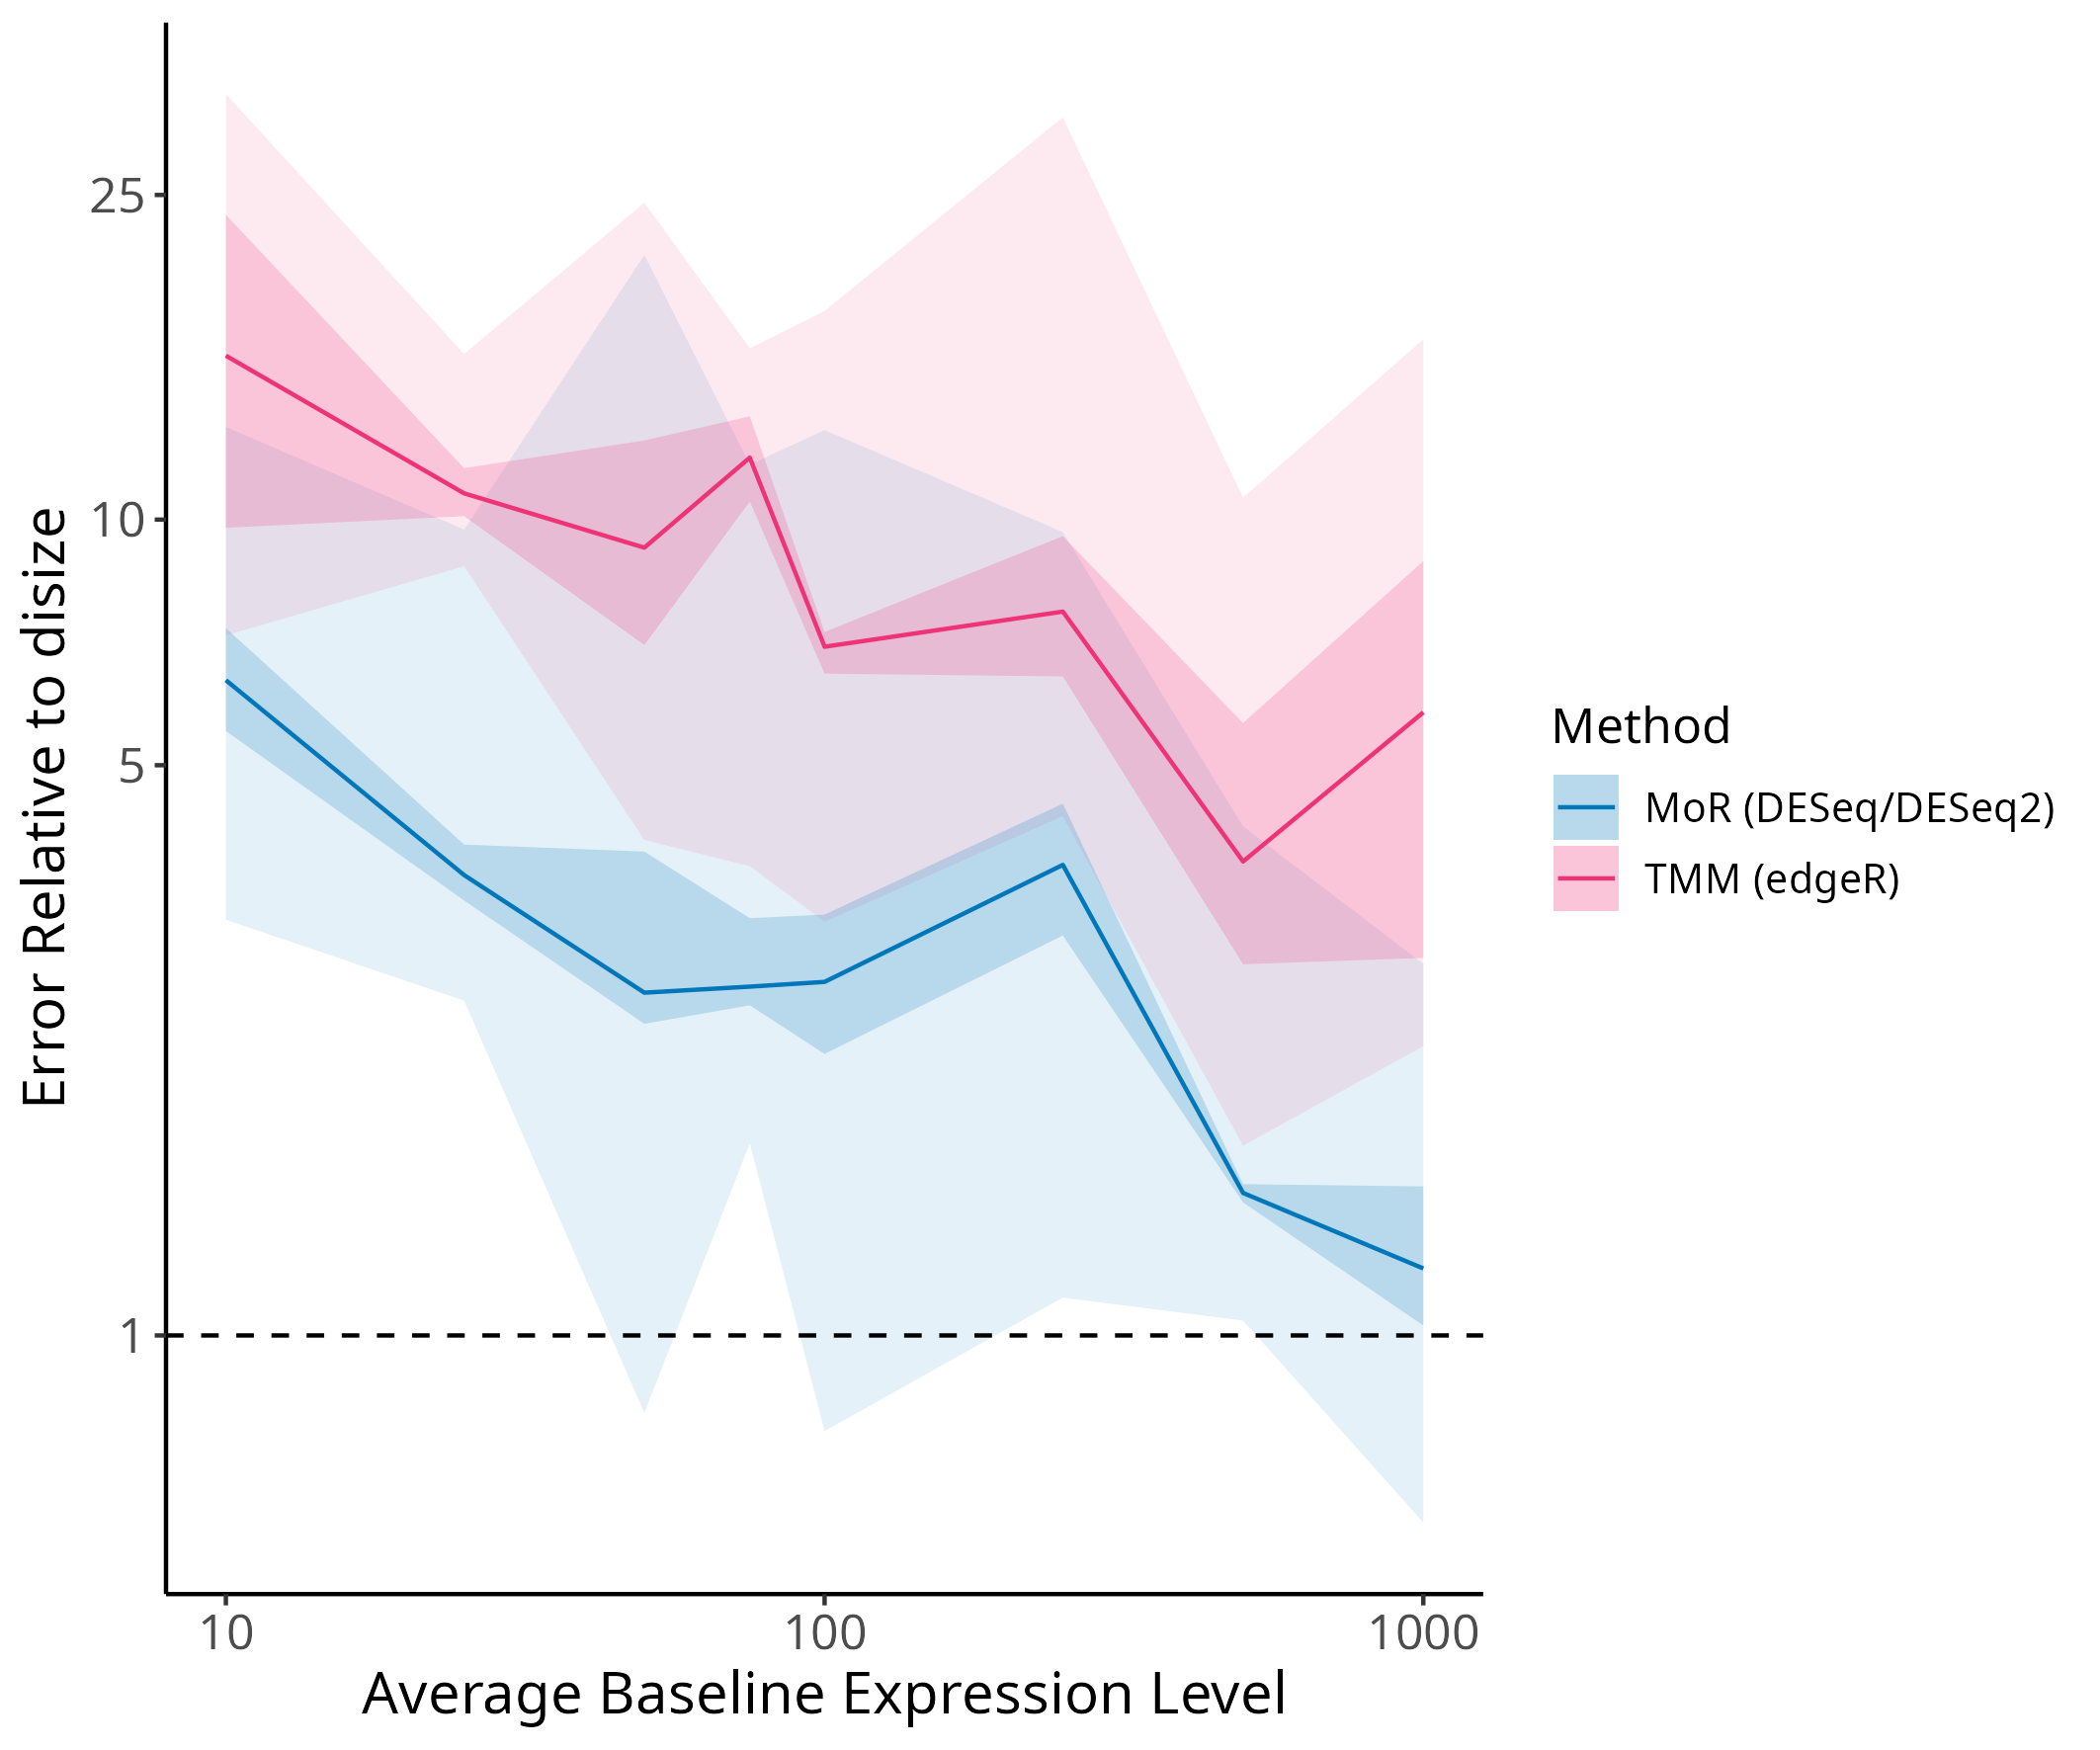
\includegraphics[width=\textwidth]{figures/fig-1-sfa.png}
\caption{
    \textbf{Comparing normalization methods for size factor accuracy across varying expression levels.}
    Fixing $n_g = 10000$, $p = 0.2$, and $\sigma = 2$ for the two-condition design, relative error in size factor estimates of MoR and TMM compared to \texttt{disize} versus the average baseline gene expression level. 
    Each line represents the median relative error, while the shaded regions indicate the 5th-95th (lighter) and 40th-60th (darker) percentile ranges. 
    A lower relative error indicates a more accurate size factor estimate.
    }
\label{fig:1}
\end{figure}

\subsection*{Impact On Downstream Analysis}

We next assessed the downstream impact of these normalization approaches on differential expression (DE) testing. 
To emulate a typical analysis workflow, we applied the size factors estimated by each method within the \verb|DESeq2| framework. 
Testing was conducted using the two-condition scenario ($10$ donors total, $5$ replicates per condition) across 100 independent simulation runs ($n_{\text{sims}} = 100$). 
We fixed the true condition effect magnitude at a high variance ($\sigma = 2.0$) while varying the baseline gene expression levels and testing across highly dense DE environments where 75\% to 85\% of genes were truly altered by the condition ($p \in \{0.15, 0.20, 0.25\}$).

As expected, using the true simulated baseline batch effects yielded the lowest Type I error rates across all baseline expression levels (\hyperref[fig:2]{Fig 2A}, S4 Fig), while the Type II error rates remained comparable across all methods (\hyperref[fig:2]{Fig 2B}, S5 Fig). The performance of the normalization methods during DE testing directly mirrored their underlying accuracy in size factor estimation, where \texttt{disize} consistently achieved the lowest Type I error compared to MoR and TMM.

\begin{figure}[H]
\centering
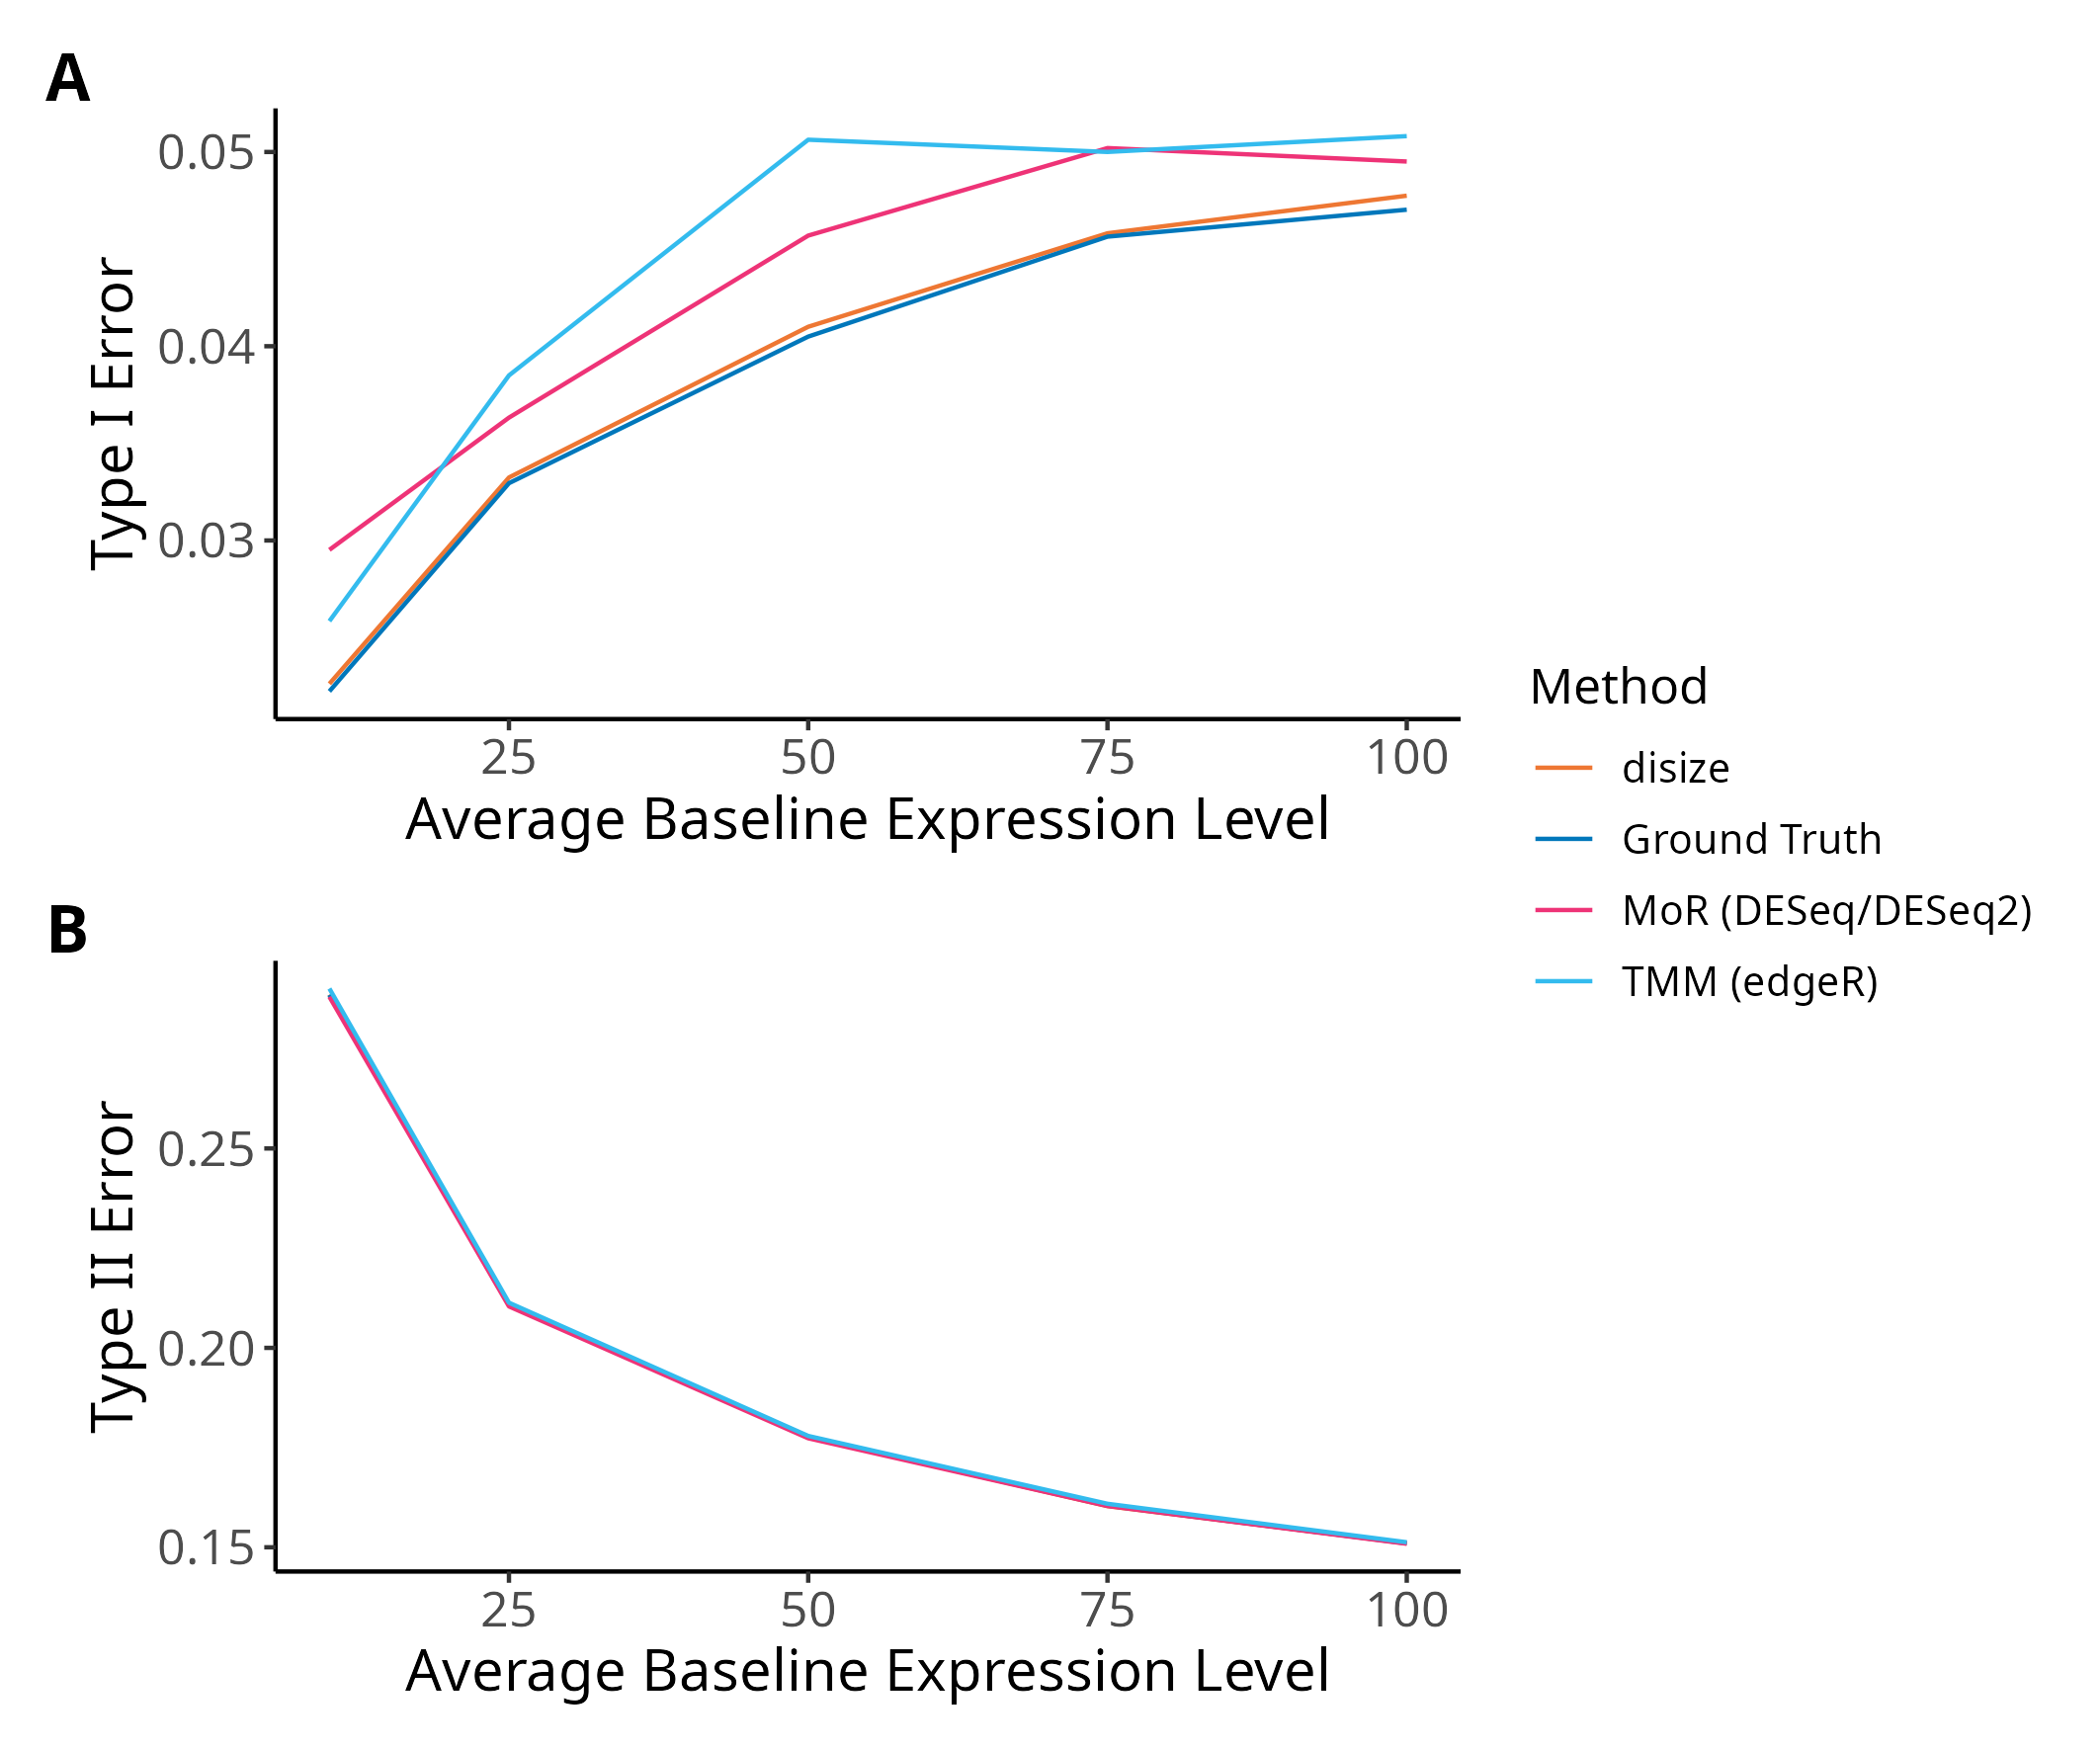
\includegraphics[width=\textwidth]{figures/fig-2-di.png}
\caption{
    \textbf{Comparing normalization methods for type I and II error across varying expression levels.}
    Fixing $n_g = 10000$, $p = 0.25$, and $\sigma = 2$ under a two-condition design (5 replicates per condition), Type I (A) and Type II (B) error rates of each normalization method (\texttt{disize}, MoR, and TMM) are plotted against the average baseline gene expression level compared to the ground truth. The nominal significance threshold is fixed at $\alpha = 0.05$.
}\label{fig:2}
\end{figure}

\subsection*{Validation With Pseudo-bulk RNA-seq Data}
To evaluate whether the performance advantages of \texttt{disize} persist when confronted with realistic count data, we tested each normalization method on pseudo-bulk data derived from a scRNA-seq dataset. We leveraged a publicly available 10x Genomics dataset consisting of 10,000 Peripheral Blood Mononuclear Cells (PBMCs) \cite{10x_genomics_10k_2020}.
Using the pre-annotated cell-type clusters as distinct biological conditions, we randomly partitioned the cells within each cluster into five batches and performed pseudo-bulking to generate expression profiles for each batch-cluster combination. 
We next used DESeq2 to perform differential expression analysis on the pseudo-bulk data where no batch effects are present, and then imposed ground-truth size factors on the expression profiles per-batch through binomial thinning. We then benchmarked how well each normalization method recovered the true size factors, the original $\text{log}_2$ fold-changes, and any genes identified as DE (defined as $p_{\text{adj}} < 0.05$ and $|\text{log}_2\ \text{fold change}| > 1$).

The pseudo-bulk evaluation closely mirrors the trends observed in our parametric simulations. 
Both MoR and TMM exhibited higher relative errors in their size factor estimates compared to \texttt{disize} (\hyperref[fig:3]{Fig~3}). 
The error in size factor accuracy directly translated to the accuracy of downstream differential expression testing. 
When evaluating downstream effects, \texttt{disize} demonstrated a lower error in $\text{log}_2$ fold-change estimates (\hyperref[fig:4]{Fig~4A}) as well as a lower Type II error rate (\hyperref[fig:4]{Fig~4B}) compared to both MoR and TMM.
This confirms that including information from cell-type annotations during normalization allows \texttt{disize} to accurately isolate batch effects in pseudo-bulk data.

\begin{figure}[H]
\centering
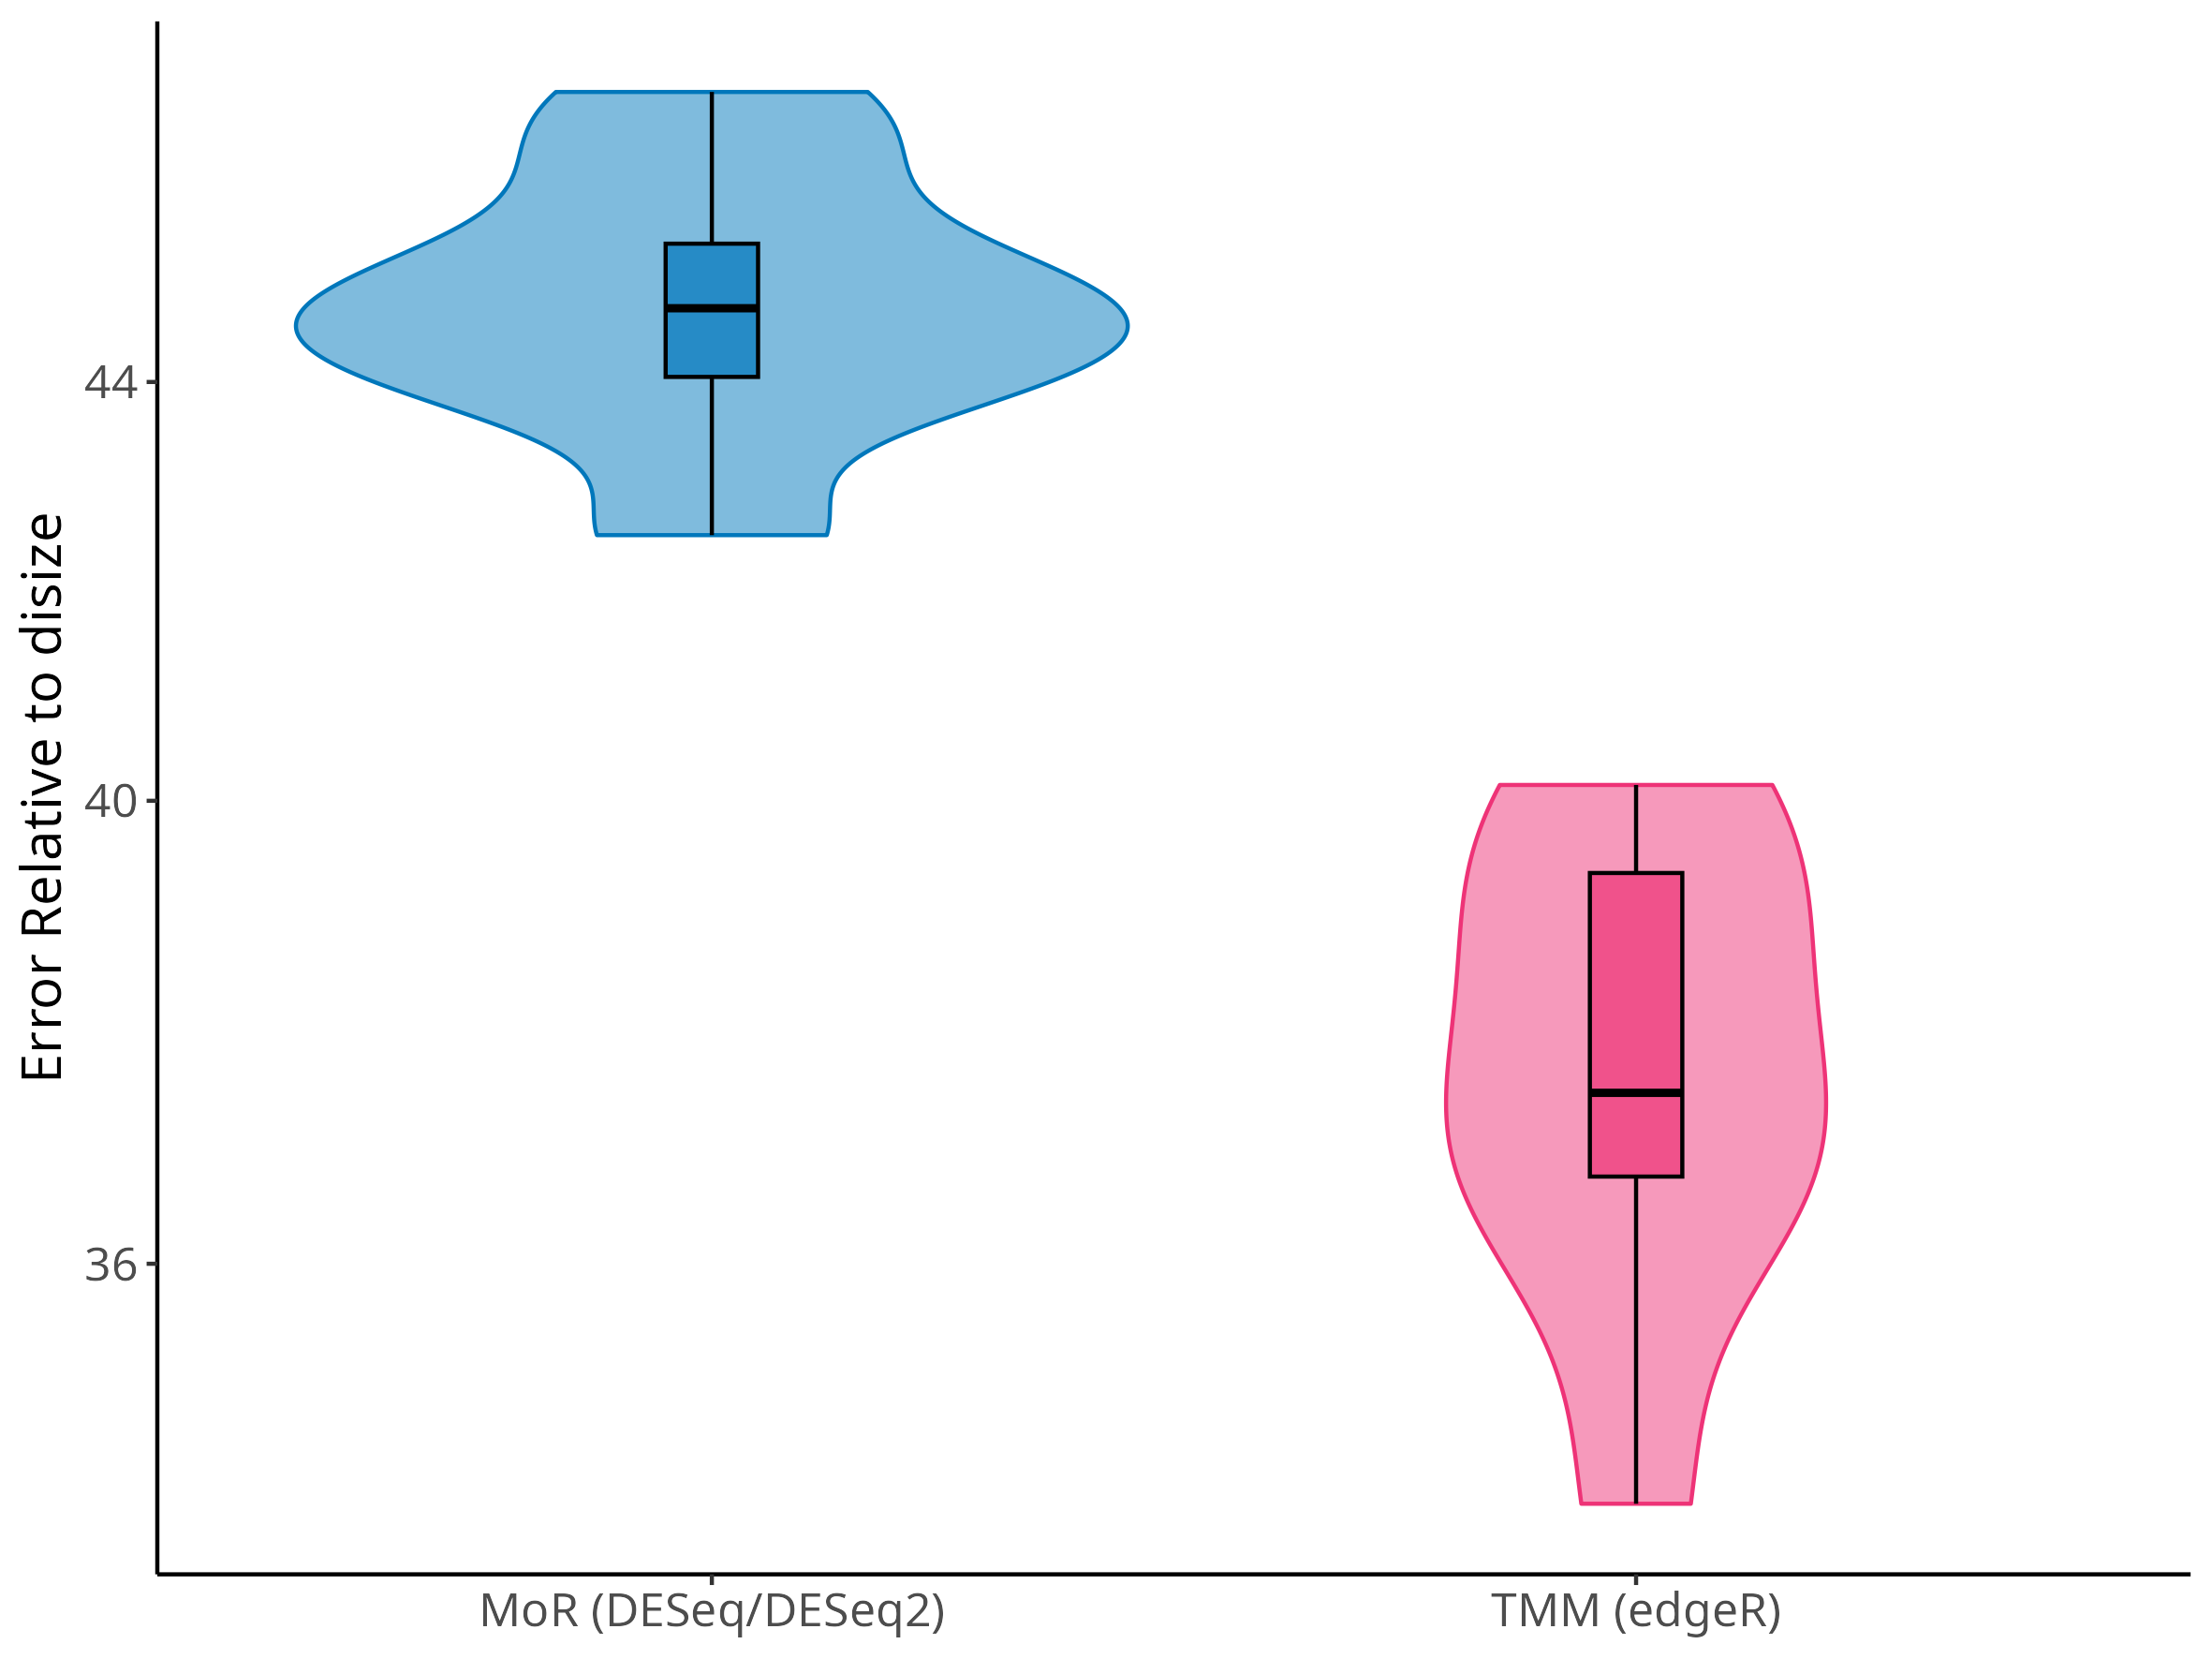
\includegraphics[width=\textwidth]{figures/fig-3-rd_sfa.png}
\caption{
    \textbf{Comparing normalization methods for size factor accuracy on pseudo-bulk data.}
    Benchmarking performance of normalization methods using pseudo-bulk data derived from human PBMC scRNA-seq data. Relative error in size factor estimates of normalization methods compared to \texttt{disize}. 
    A lower relative error indicates a more accurate recovery of the imposed batch effects.
}\label{fig:3}
\end{figure}

\begin{figure}[H]
\centering
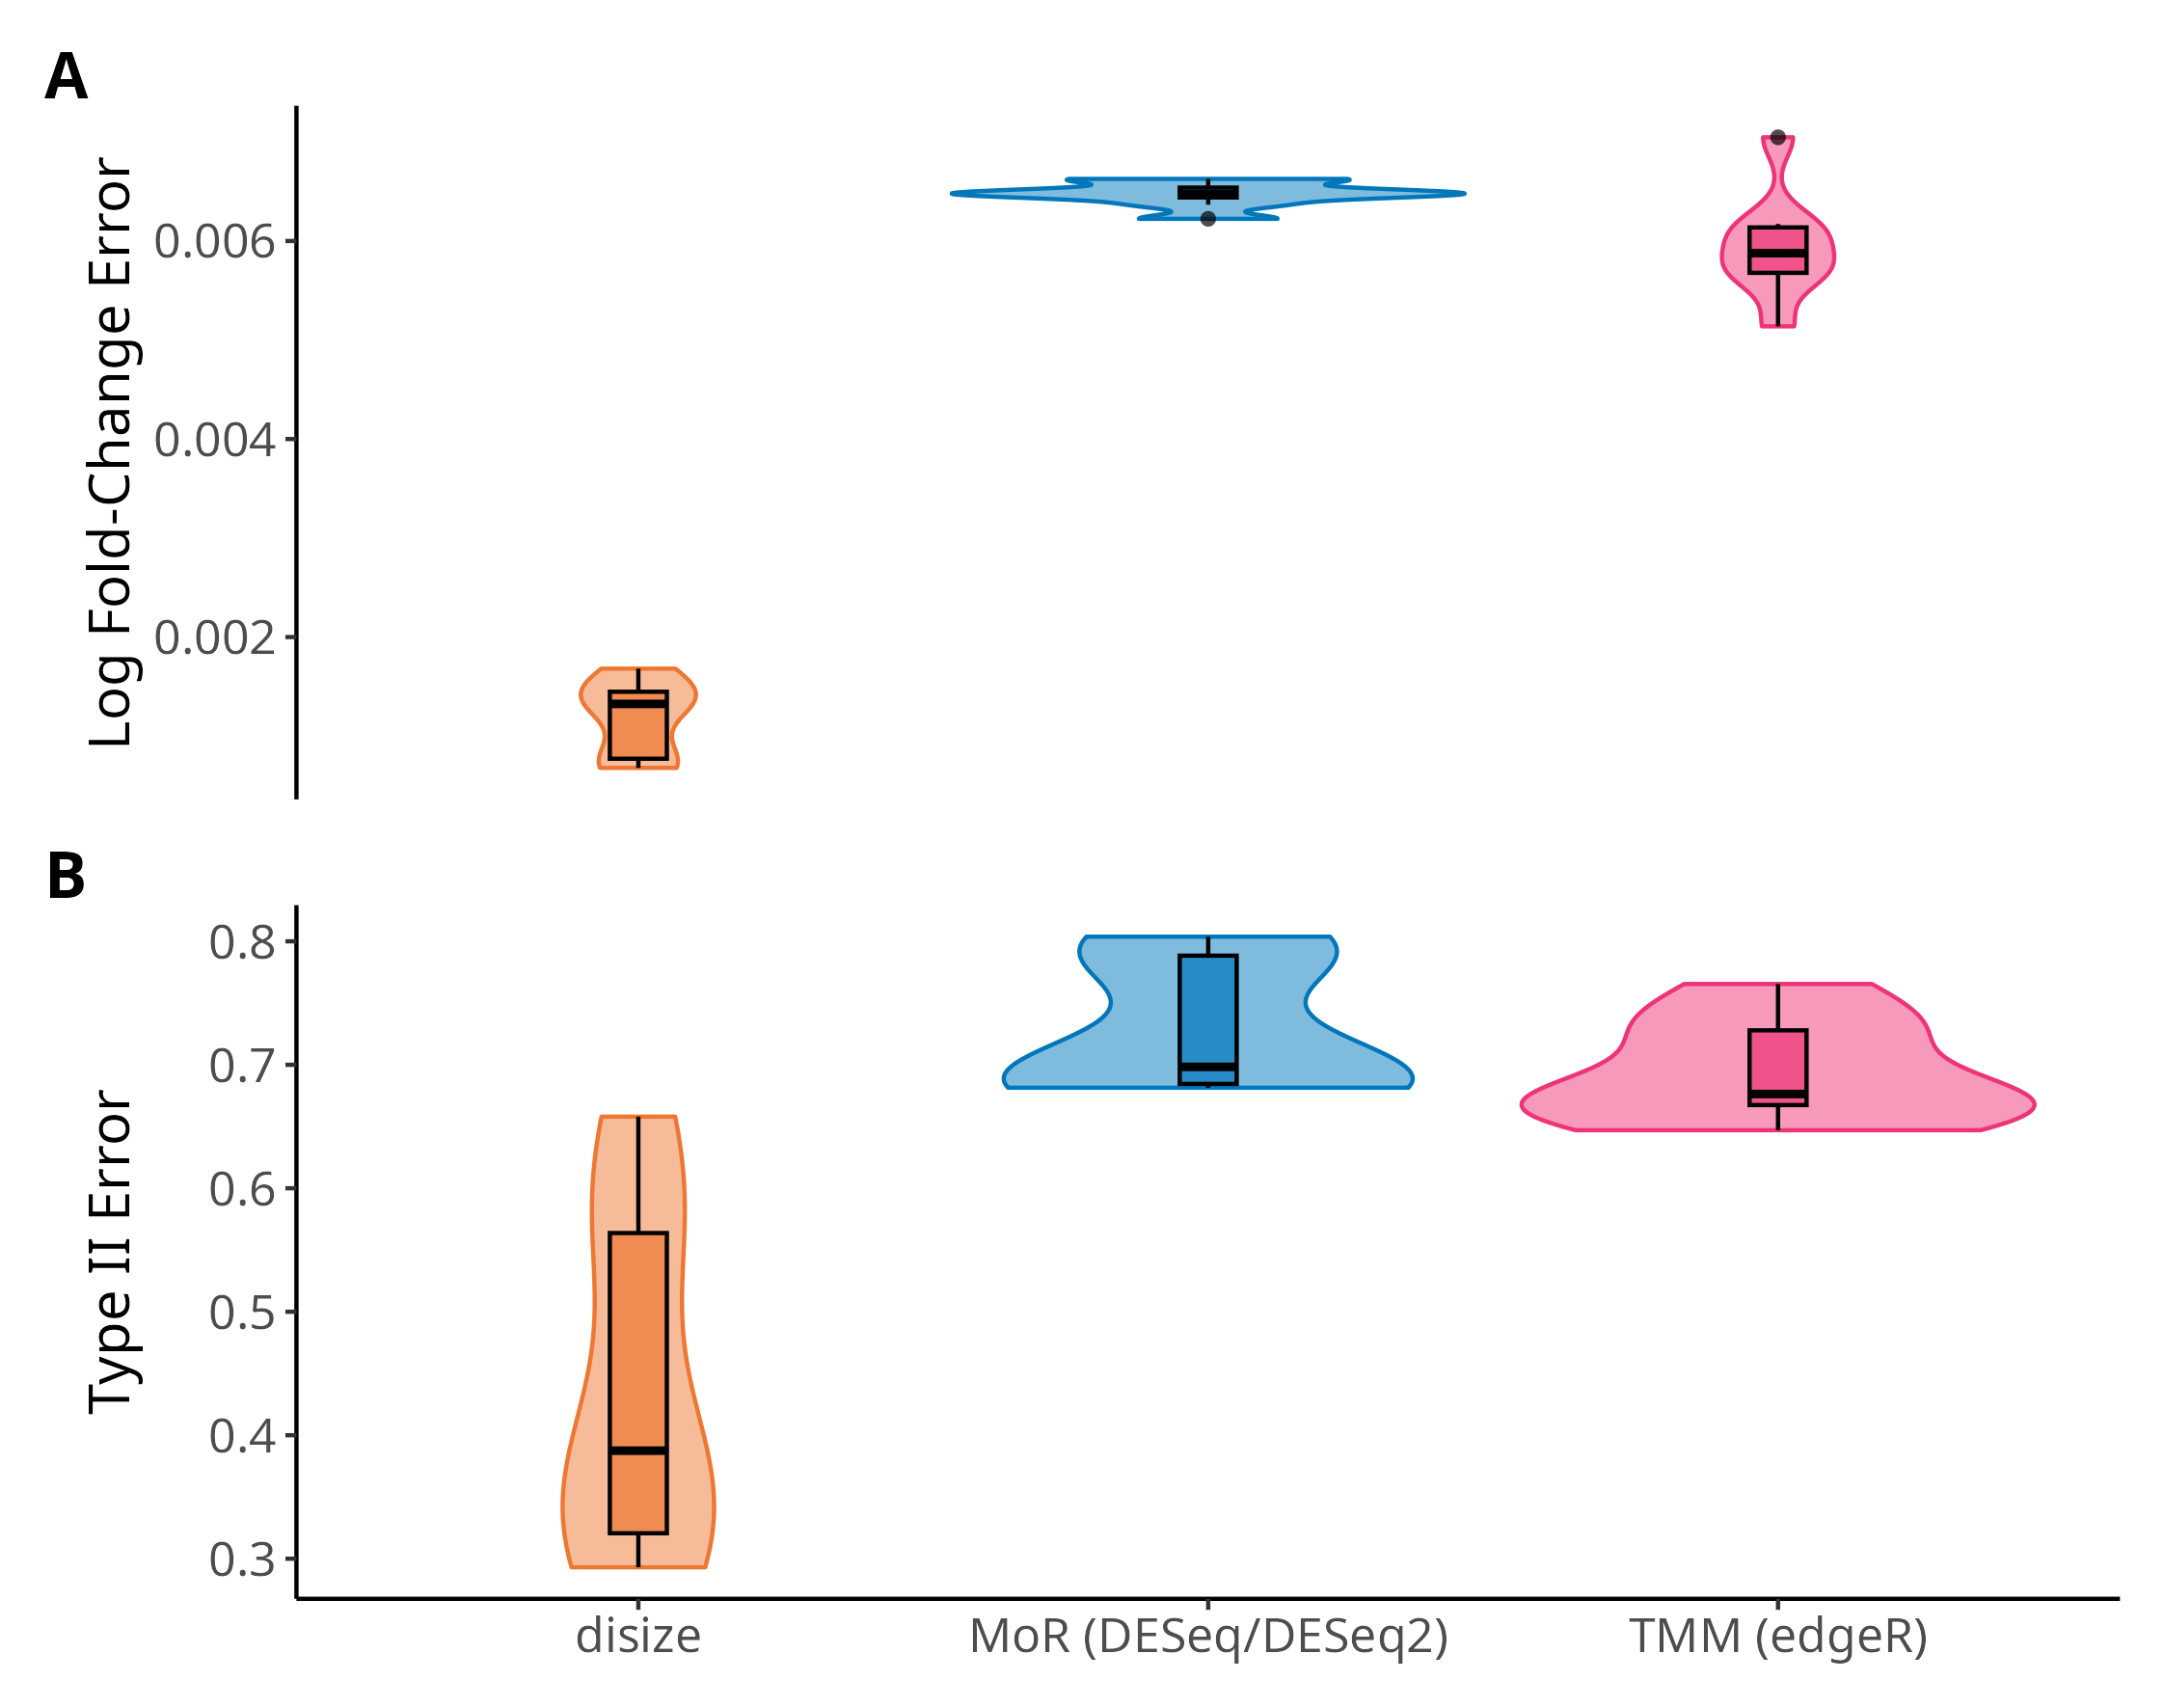
\includegraphics[width=\textwidth]{figures/fig-4-rd_dea.png}
\caption{
    \textbf{Comparing normalization methods for downstream differential expression analysis on pseudo-bulk data.}
    Benchmarking performance of normalization methods using pseudo-bulk data derived from human PBMC scRNA-seq data. 
    (A) Downstream absolute error in $\text{log}_2$ fold-change estimates of normalization methods compared to \texttt{disize} in the contrast between clusters 6 and 7. 
    (B) Downstream Type II error of normalization methods compared to \texttt{disize} in the contrast between clusters 6 and 7. 
    A lower error indicates a more accurate recovery of the true differential expression.
}\label{fig:4}
\end{figure}

\subsection*{A Case Study of scRNA-seq Data From Interferon-$\beta$ Stimulated PBMCs}

To evaluate its utility on multi-donor single-cell experiments, we applied \texttt{disize} to a scRNA-seq dataset of human PBMCs stimulated with interferon-beta (IFN-$\beta$) or left untreated as controls \cite{kang_multiplexed_2018}.
We aggregated the single-cell counts into pseudo-bulk profiles stratified by experimental condition, donor identity, and cell-type annotation, yielding a multi-factorial experimental design with a varying number of cells contributing to each pseudo-bulk sample. 
We then estimated size factors for each sample, where \texttt{disize} was supplied the experimental design with an interaction between the condition and cell-type annotation, and the log-transformed number of cells contributing to each pseudo-bulk sample as offsets.

Using each set of size factors, we conducted cell-type-specific DE testing with \verb|DESeq2| by specifying an interaction between the condition and cell-type annotation to compare the IFN-$\beta$ stimulated group against the control baseline within each annotated group. 
Significant differentially expressed genes (DEGs) were identified using a threshold of $p_{\text{adj}} < 0.05$ and $|\text{log}_2 \text{fold change}| > 1$.

Across the majority of the 13 cell types, \texttt{disize} consistently identified a larger number of significant DEGs compared to MoR and TMM (\hyperref[fig:5]{Fig~5}). 
Notably, this trend was most pronounced in CD14+ monocytes, which yielded the highest absolute number of DEGs discovered by \texttt{disize} (\hyperref[fig:6]{Fig~6}).
The increased sensitivity relative to other normalization methods indicates that \texttt{disize} is particularly useful for scRNA-seq experiments. 

\begin{figure}[H]
\centering
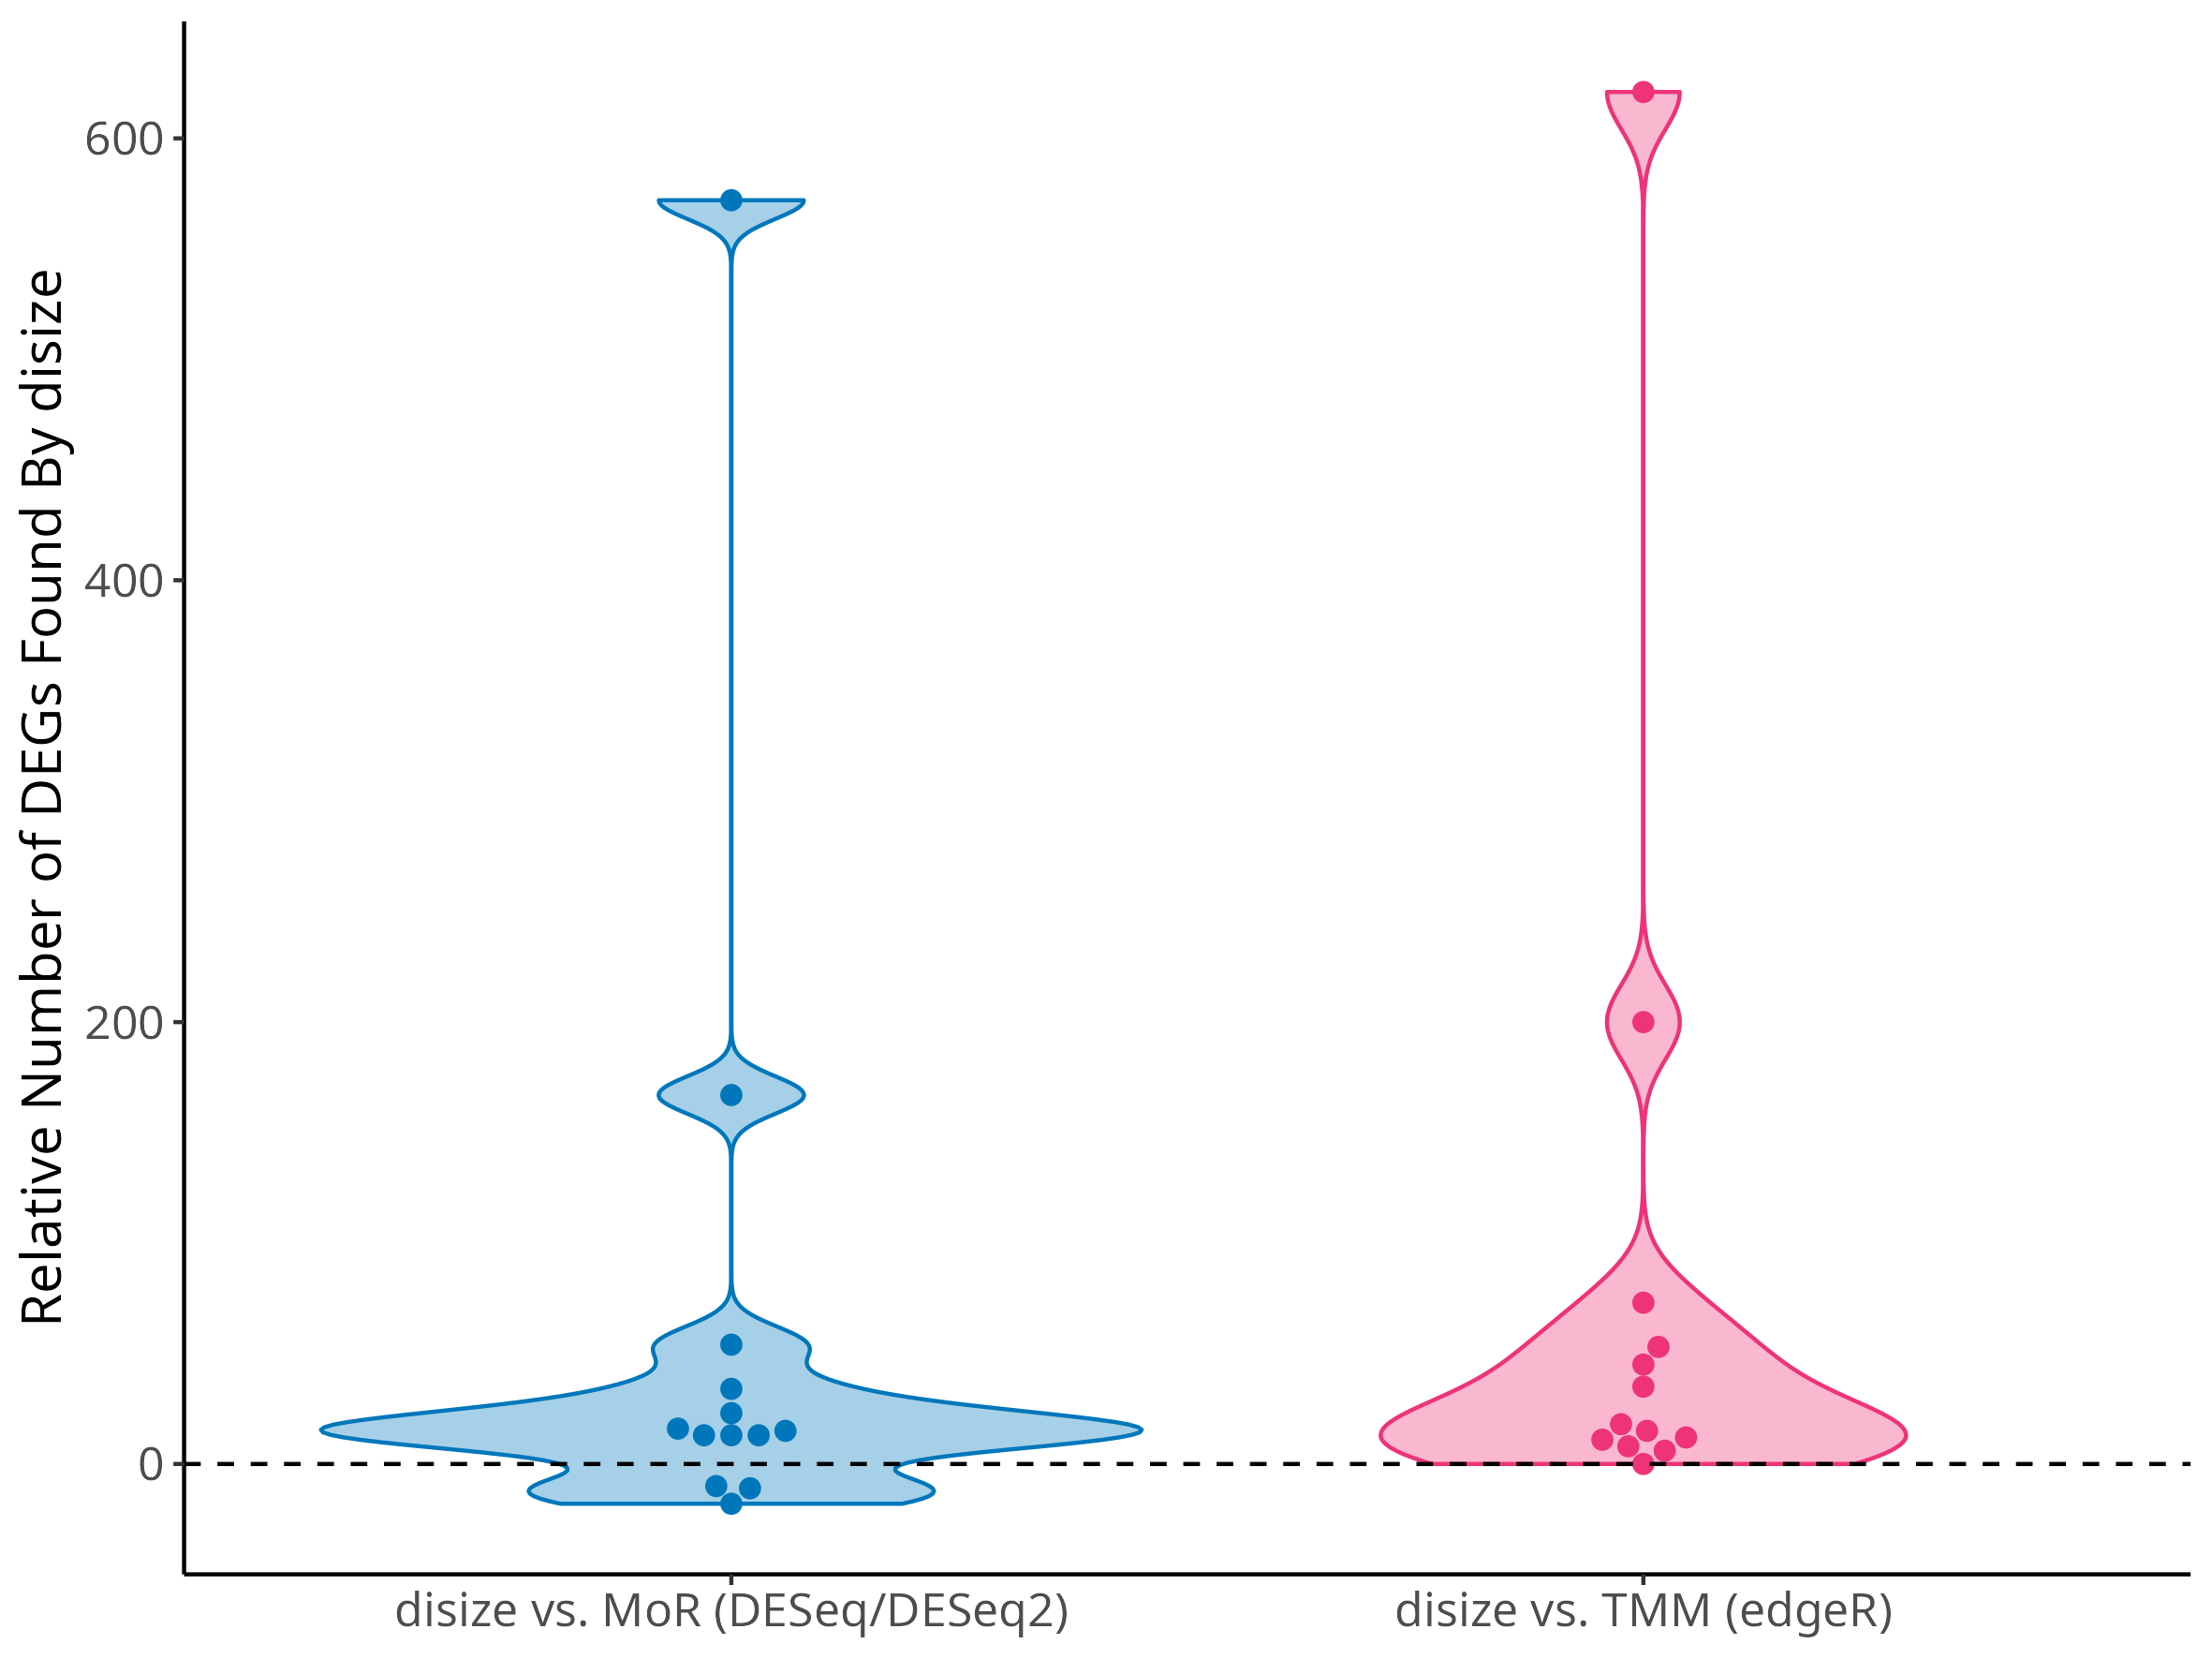
\includegraphics[width=\textwidth]{figures/fig-5-sc.png}
\caption{
    \textbf{Comparison of identified differentially expressed genes across normalization methods in empirical IFN-$\beta$ stimulated pseudo-bulk data.} 
    Relative gain in identified DEGs between conditions ($p_{\text{adj}} < 0.05$, $|\log_2 \text{fold-change}| > 1$) for each of the 13 cell types when utilizing \texttt{disize}, calculated as the difference in the number of discovered DEGs compared directly to MoR and TMM. Positive values indicate a higher number of significant genes discovered by \texttt{disize}.
}\label{fig:5}
\end{figure}

\begin{figure}[H]
\centering
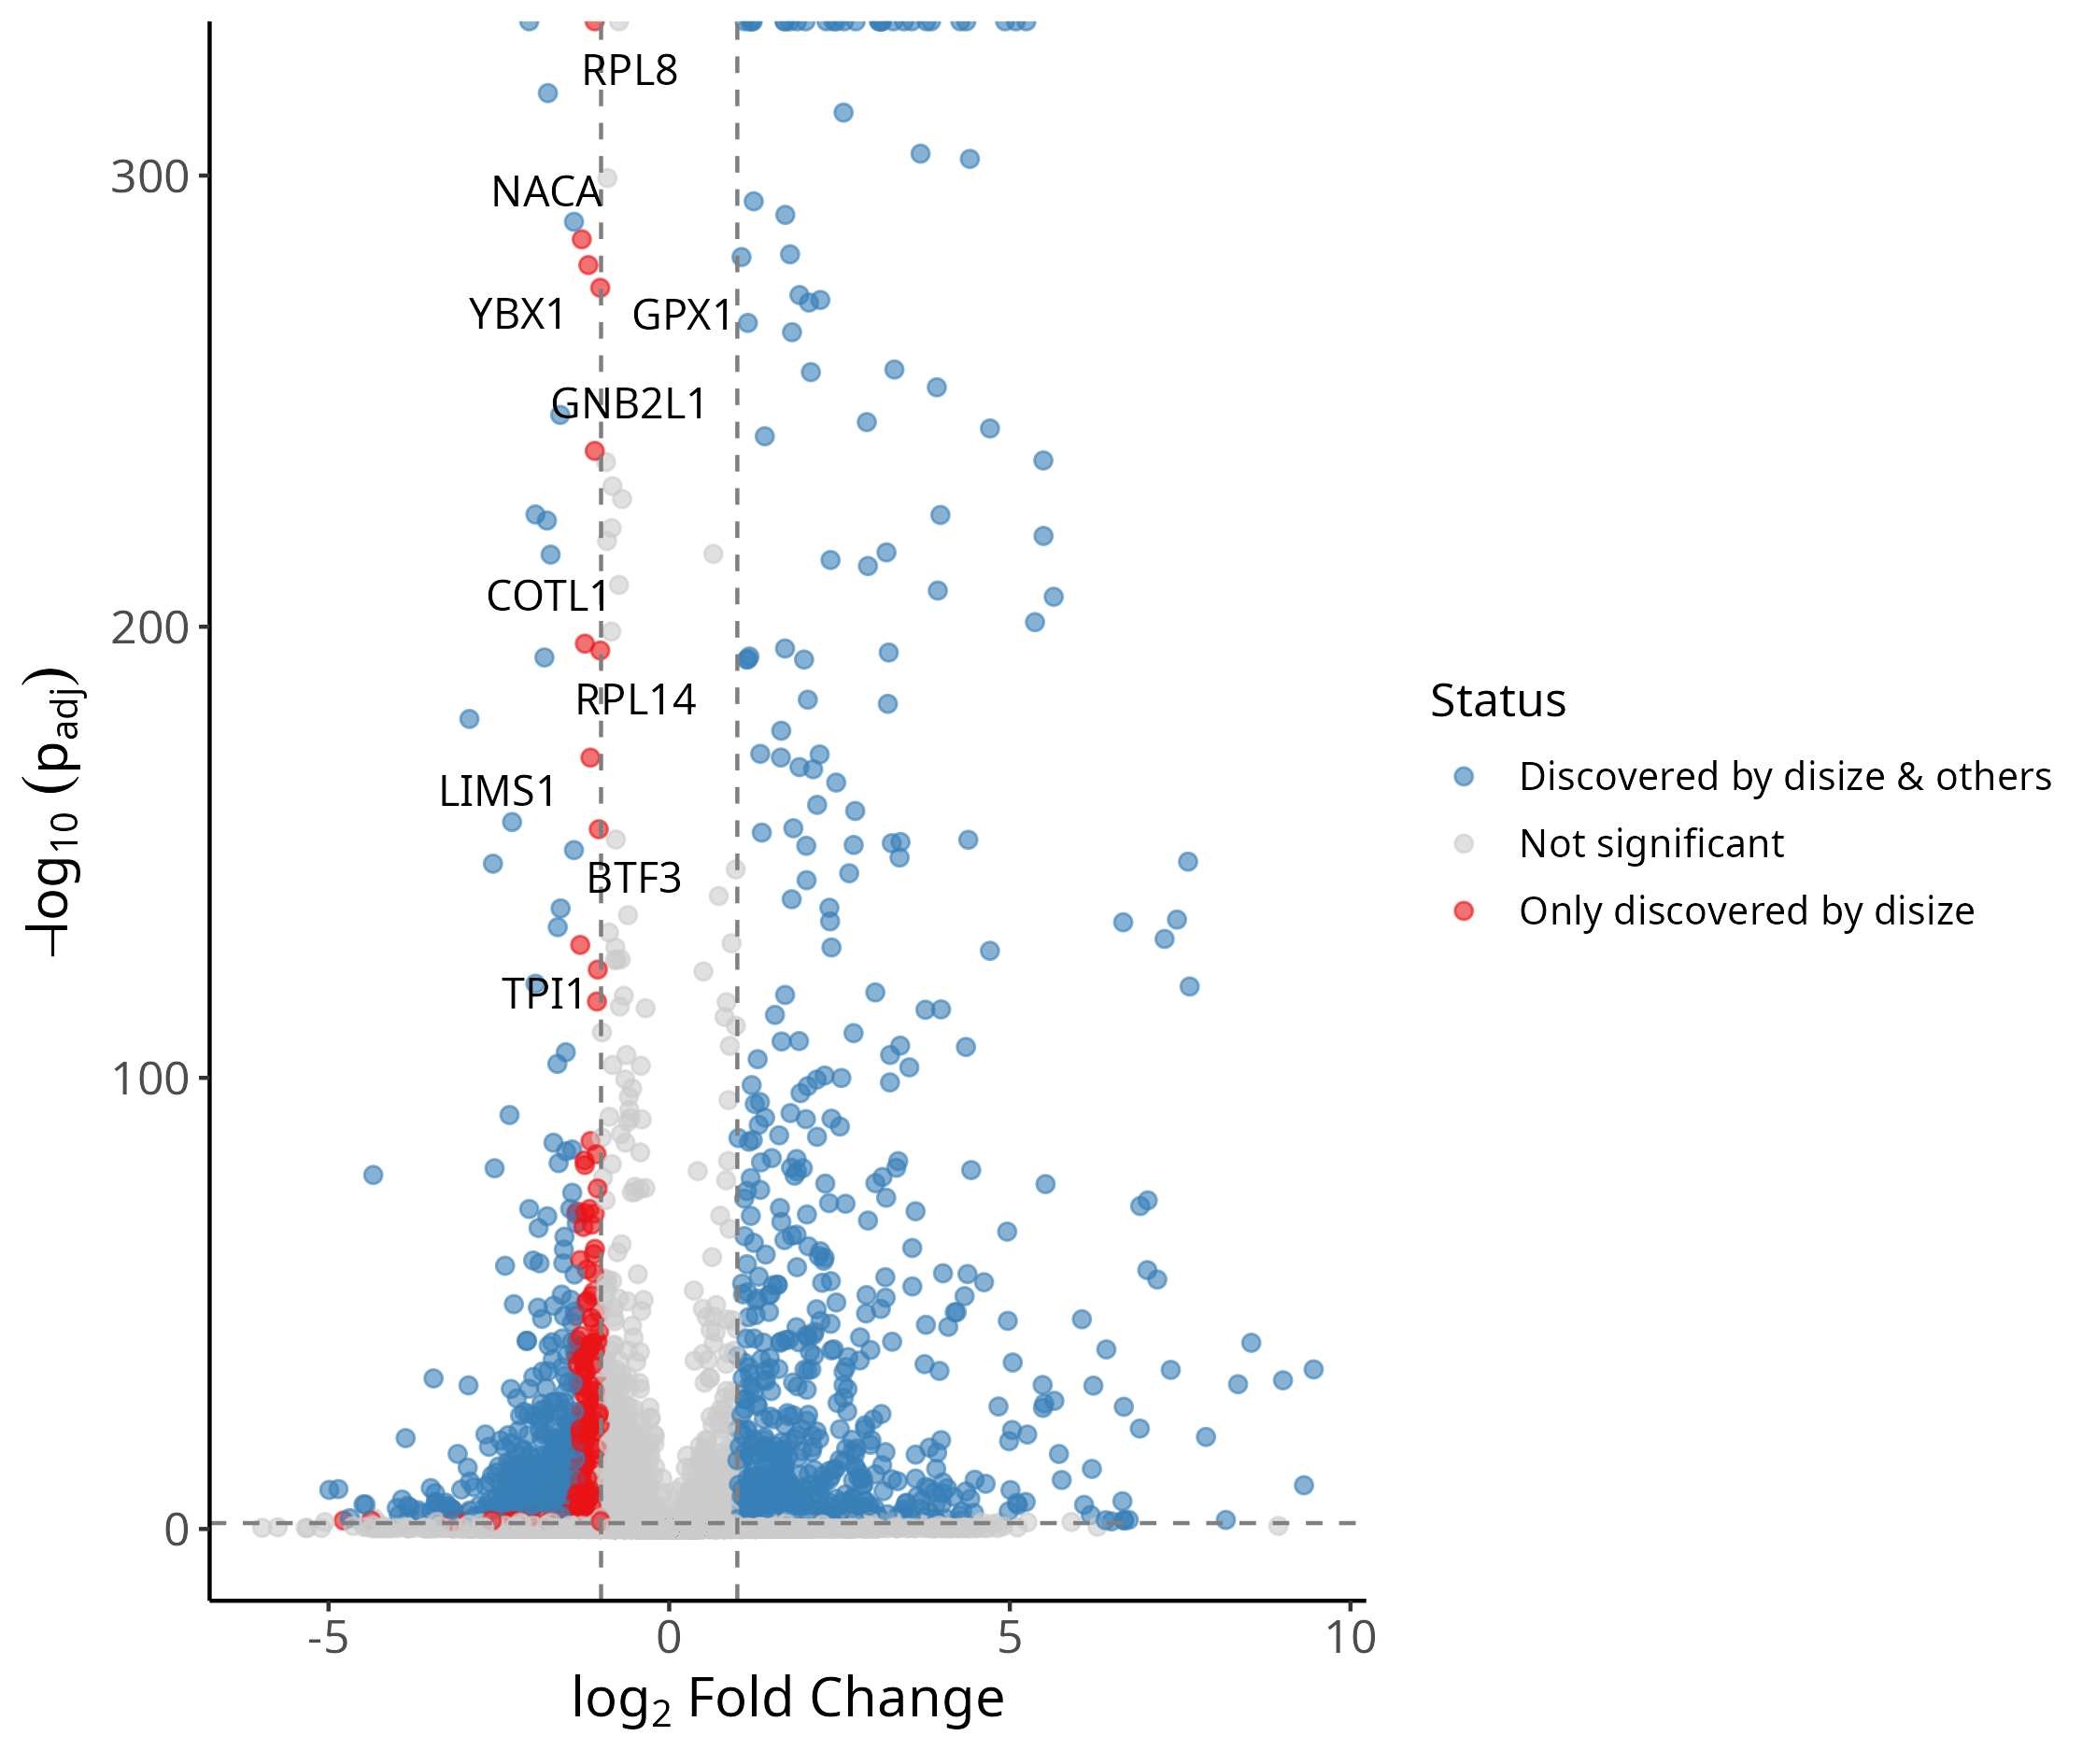
\includegraphics[width=\textwidth]{figures/fig-6-sc-vp.png}
\caption{
    \textbf{Volcano plot of differential gene expression in CD14+ monocytes normalized via \texttt{disize}.} 
    Points represent individual genes plotted by their $\text{log}_2$ fold change (IFN-$\beta$ stimulated relative to control baseline) and statistical significance ($-\log_{10} p_{\text{adj}}$). 
    Genes identified as significant by both \texttt{disize} and alternative normalization methods (MoR/TMM) are shown in blue; genes falling below the significance thresholds ($p_{\text{adj}} \ge 0.05$ or $|\text{log}_2\ \text{fold-change}| \le 1.0$) are shown in grey; and genes uniquely resolved as significant by \texttt{disize} are shown in red. 
    The top 10 unique \texttt{disize} discoveries by $p_{\text{adj}}$ are labeled.
}\label{fig:6}
\end{figure}

\section*{Discussion}

While researchers have made significant progress in RNA-seq analysis, much of this work has focused on improving downstream DE testing, with less attention paid to the preceding step of normalization. 
We address this gap by proposing a novel normalization method that explicitly leverages information from the experimental design to improve the accuracy of size factor estimation.

Our benchmarking demonstrates that \texttt{disize} works well under various scenarios, particularly those with non-trivial biological variation across experimental units, low sparsity (i.e., a high proportion of DE genes), and many genes with low expression.
This makes \texttt{disize} particularly well suited for single-cell RNA-seq (scRNA-seq) analysis, where pseudo-bulking (aggregating counts from multiple cells into a single ``sample'') may not accumulate enough counts for other methods to work effectively, and the biological differences between cell types can result in little sparsity.
Indeed, \texttt{disize} greatly outperformed both MoR and TMM in our pseudo-bulk evaluation and recovered more DEGs than MoR and TMM in the case study of IFN-$\beta$ stimulated PBMCs, demonstrating that our method successfully leverages information in cell-type annotations to improve size factor estimation.

Although the Type II error rates were comparable across methods in the parametric simulation benchmarks, since \texttt{disize} had the lowest Type I error rate---often below the nominal $\alpha = 0.05$ for low baseline expression---there is potential for increasing the specified significance threshold to produce a lower Type II error rate while retaining a Type I error below the desired $\alpha$.
In simpler experiments, however, MoR normalization is roughly as accurate as \texttt{disize} when most genes have sufficient expression ($> 100$ counts) and large systematic biological variation is unlikely.

Previous benchmarks of normalization methods \cite{robinson_scaling_2010, li_choice_2020} have simulated data by drawing from a multinomial distribution, where the total number of trials represents the library size and a specified vector of probabilities defines the gene expression profile. 
While this approach is convenient, it fails to account for the overdispersion present in RNA-seq data and lacks a realistic mechanism describing how sample preparation and sequencing imperfectly measure the true number of transcripts resulting in the observed count.
We offer an alternative DGP that explicitly models the original magnitude of gene expression and the total effect of technical factors on the observed count distribution.

Since \texttt{disize} jointly estimates the effect of covariates on gene expression and the batch effect, performing inference on the full model may be useful to combine normalization and differential expression quantification into a single step.
Currently, we discard the point estimates for the covariate coefficients specified by the experimental design, and do not quantify uncertainty for any parameters.
Although the model is complex to fit due to the large number of features in transcriptomic experiments, variational inference methods could approximate the posterior distribution efficiently \cite{blei_variational_2017}. 
This full model would enable differential expression analysis without an explicit normalization step and would quantify uncertainty in size factor estimates.

Although this work has focused on bulk and pseudo-bulk scenarios, since \texttt{disize} allows for an arbitrary batch membership structure, normalization could be done directly with scRNA-seq data. 
This approach leverages the fact that cells belonging to the same sample share a batch effect (avoiding the need for offsets when pseudo-bulking). 
Consequently, using \texttt{disize} with tools specifically developed for DE testing in single-cell experiments (such as glmGamPoi \cite{ahlmann-eltze_glmgampoi_2021}) a pseudo-bulking step could be avoided altogether. 
However, a potential issue with the current implementation is that \texttt{disize} represents the count matrix in a dense format, which increases the memory footprint and may preclude its use with large datasets. 
Future work could allow a sparse representation, which would significantly reduce the memory requirements.


\section*{Supporting information}

% Include only the SI item label in the paragraph heading. Use the \nameref{label} command to cite SI items in the text.
\begin{figure}[!ht]
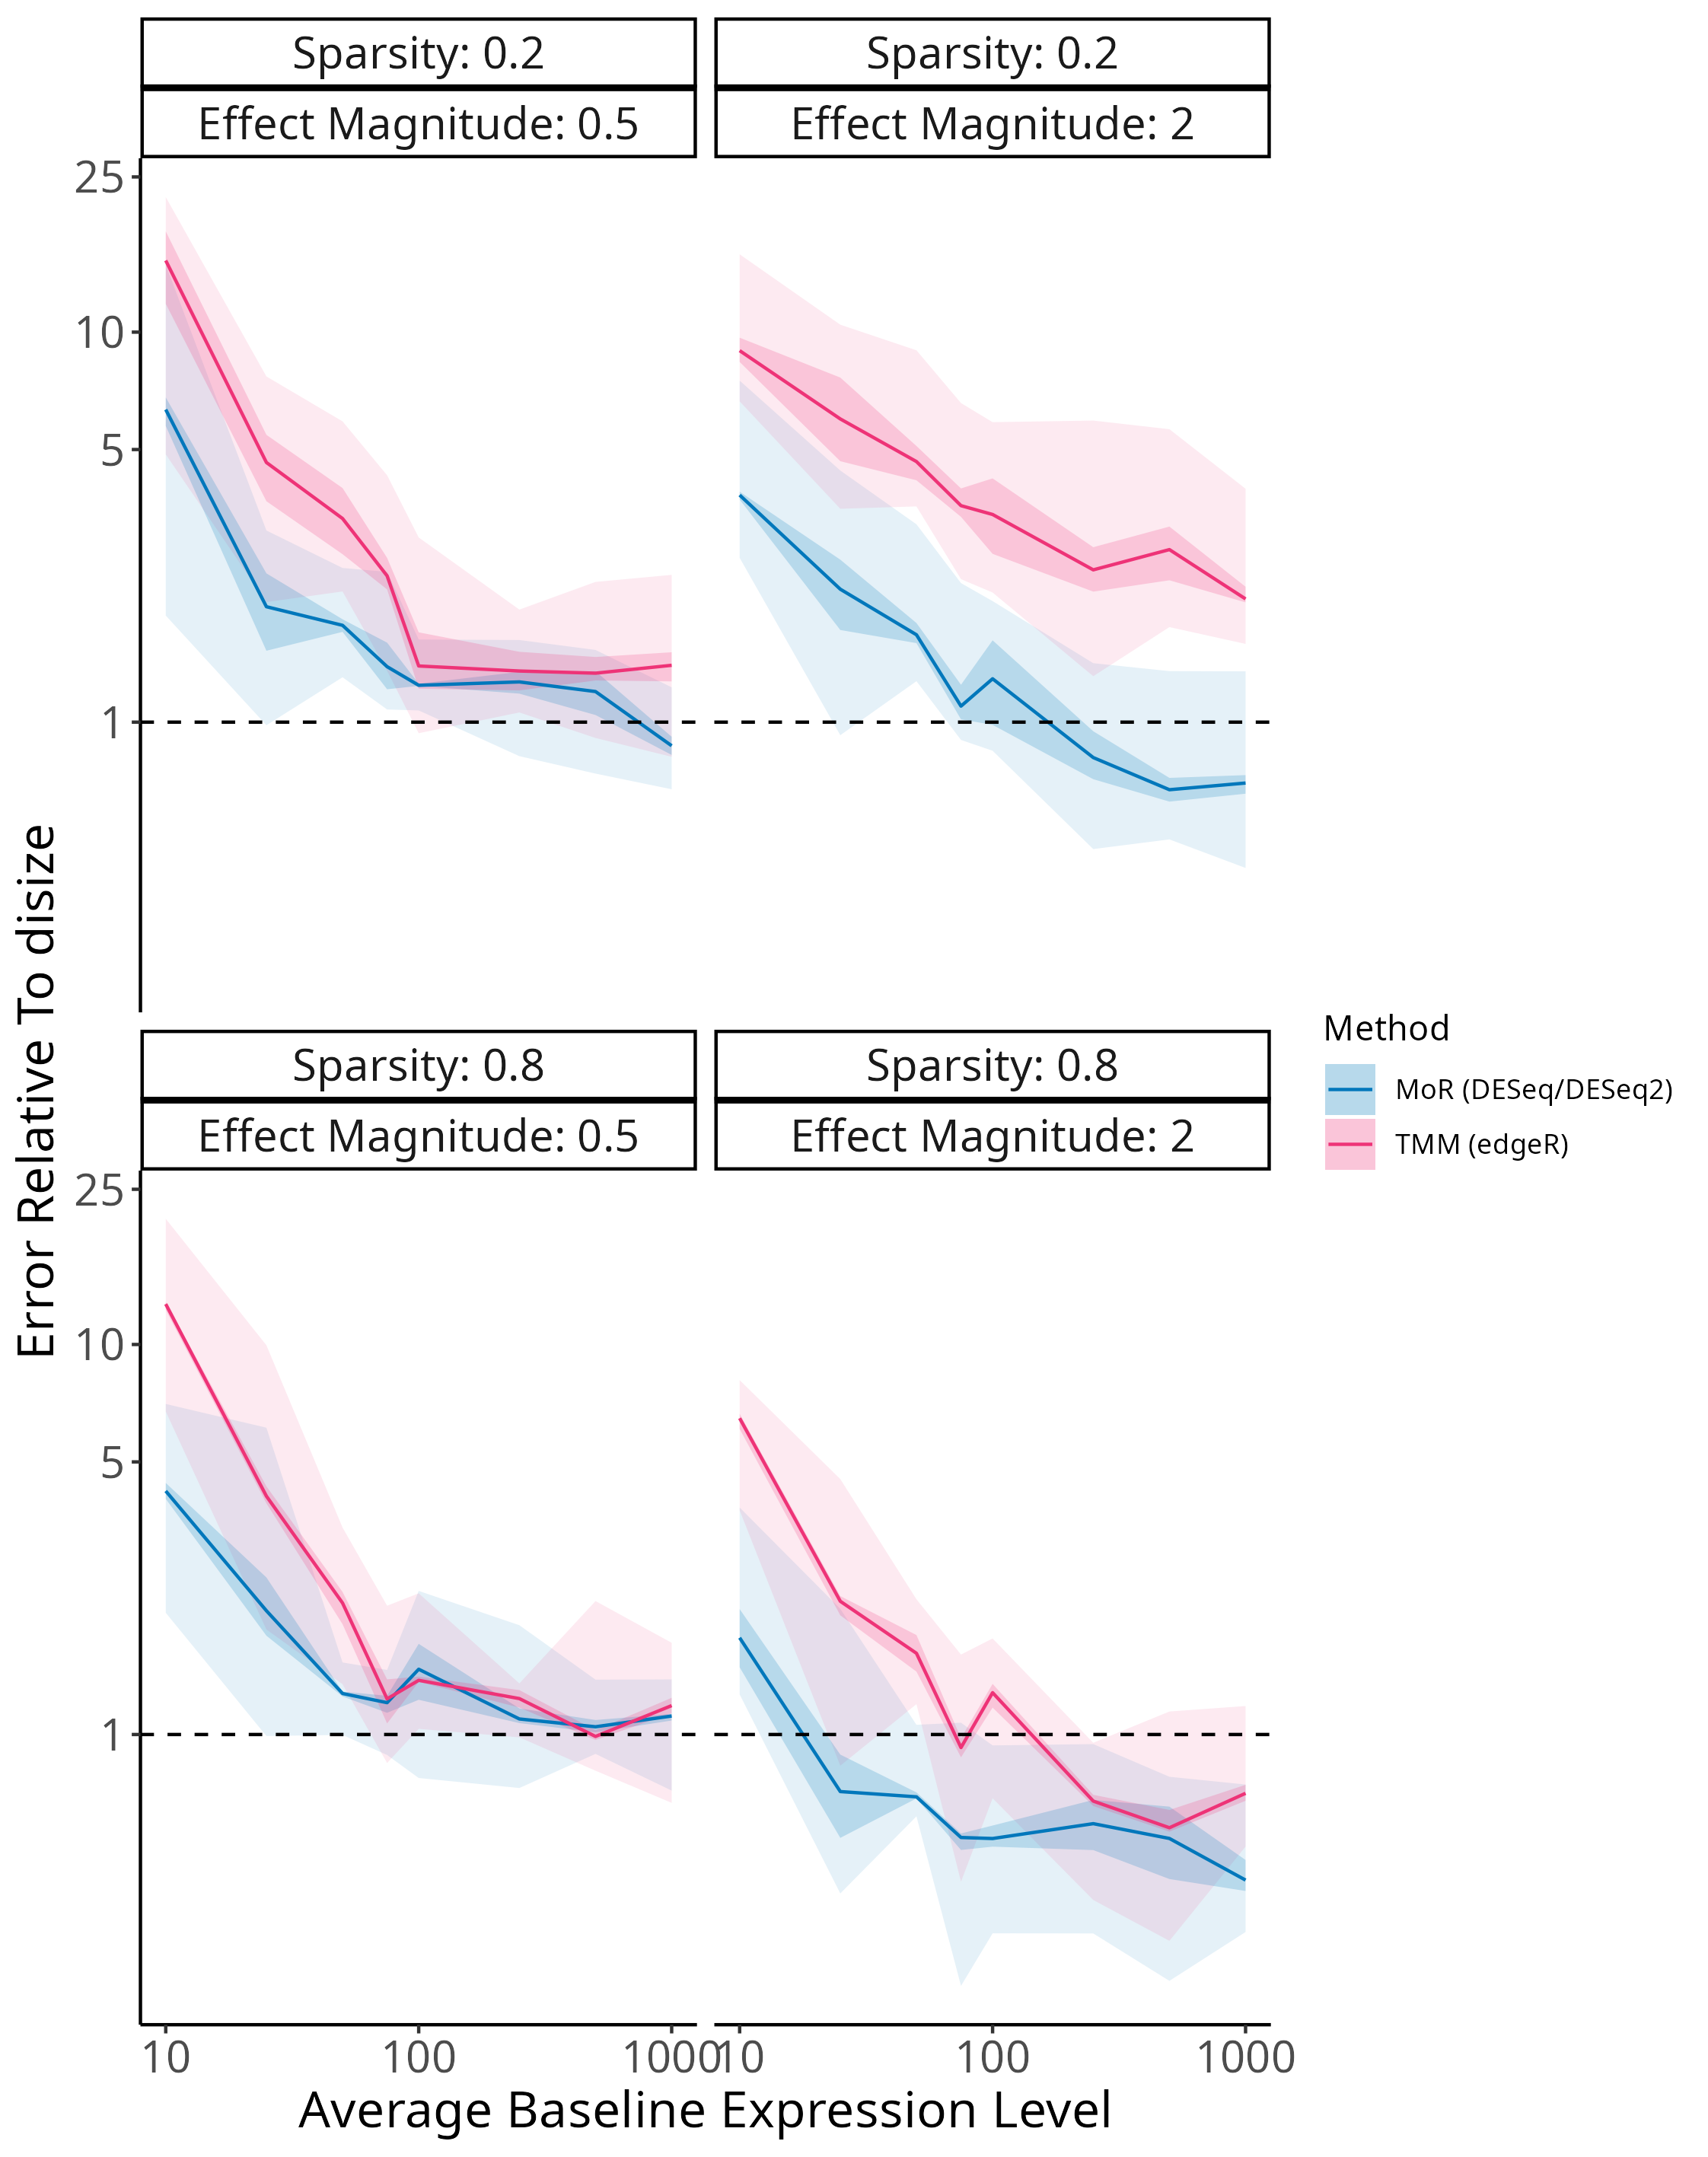
\includegraphics[width=\textwidth]{figures/suppfig-sfa-1.png}
\paragraph*{S1 Fig.}
\textbf{Comparing normalization methods for size factor accuracy in a trivial design.} 
Fixing $n_g = 10000$ and varying $p$ and $\sigma$, relative size factor error of the other normalization methods (MoR and TMM) compared to \texttt{disize} versus the average baseline gene expression level. 
Each line represents the median relative error, while the shaded regions indicate the 5th-95th (lighter) and 40th-60th (darker) percentile ranges. 
A lower relative error indicates a more accurate size factor estimate.
\end{figure}

\begin{figure}[!ht]
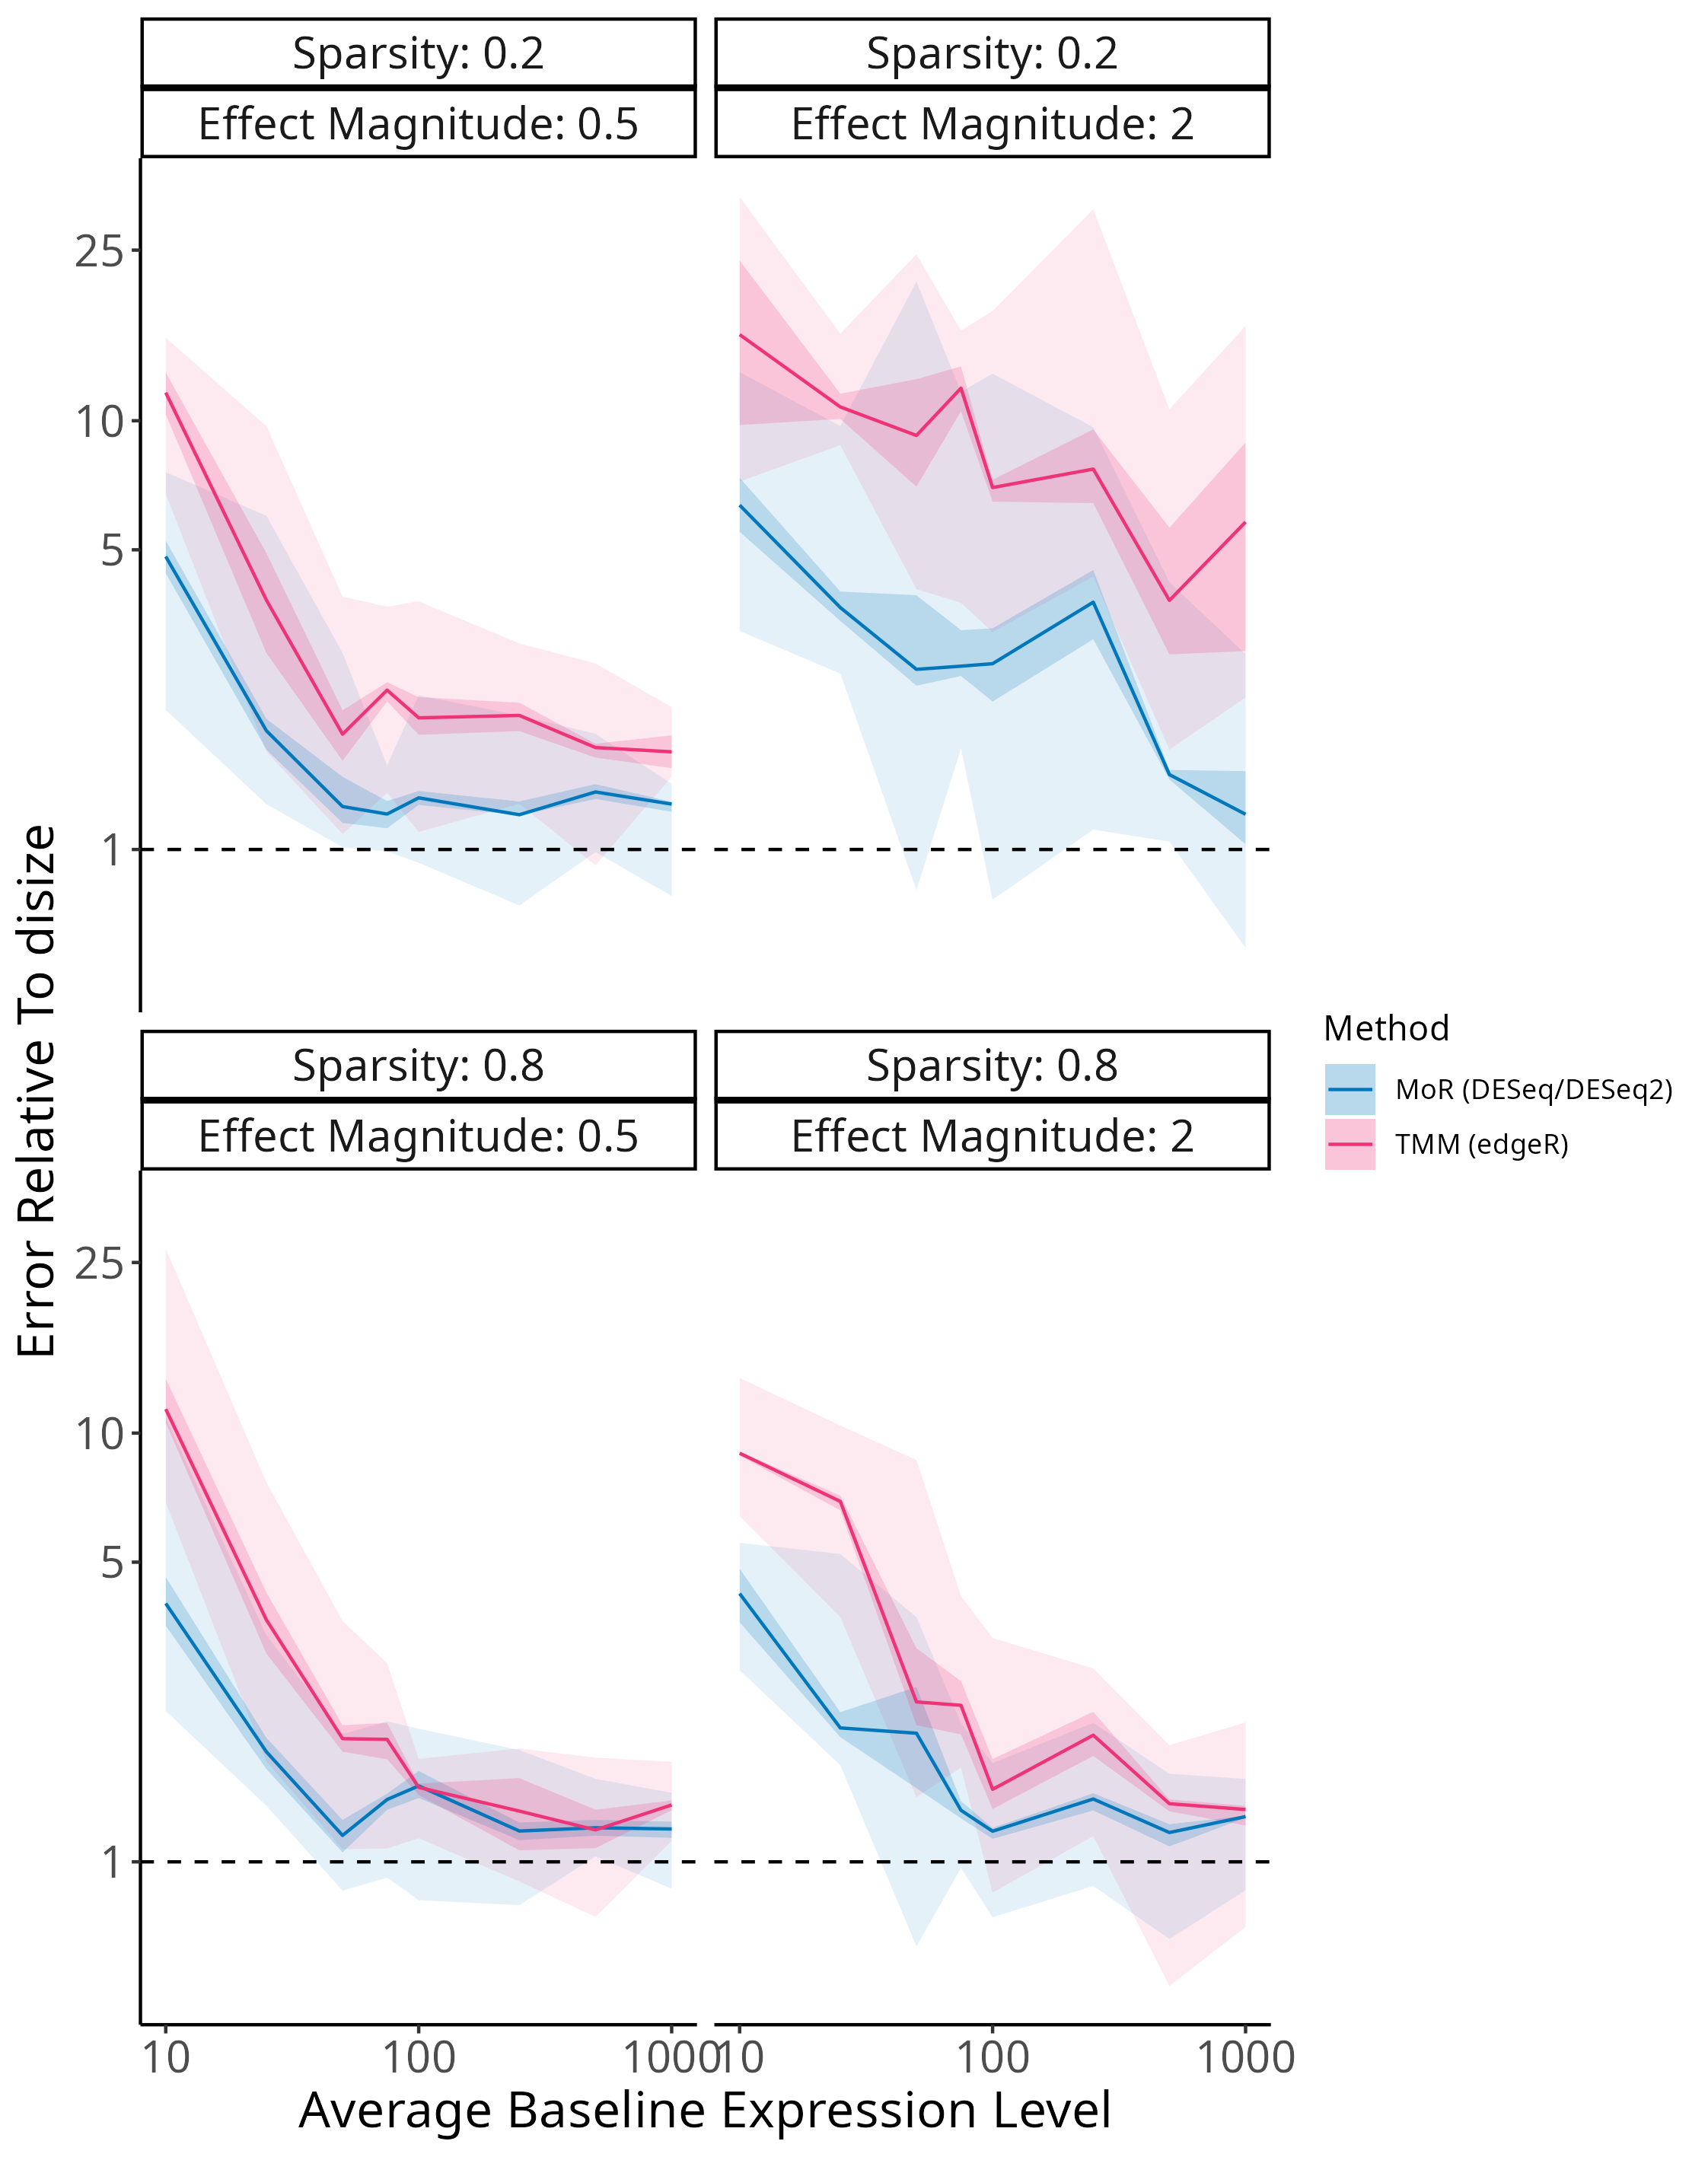
\includegraphics[width=\textwidth]{figures/suppfig-sfa-2.png}
\paragraph*{S2 Fig.}
\textbf{Comparing normalization methods for size factor accuracy in a two-group design.}
Fixing $n_g = 10000$ and varying $p$ and $\sigma$, relative size factor error of the other normalization methods (MoR and TMM) compared to \texttt{disize} versus the average baseline gene expression level. 
Each line represents the median relative error, while the shaded regions indicate the 5th-95th (lighter) and 40th-60th (darker) percentile ranges. 
A lower relative error indicates a more accurate size factor estimate.
\end{figure}

\begin{figure}[!ht]
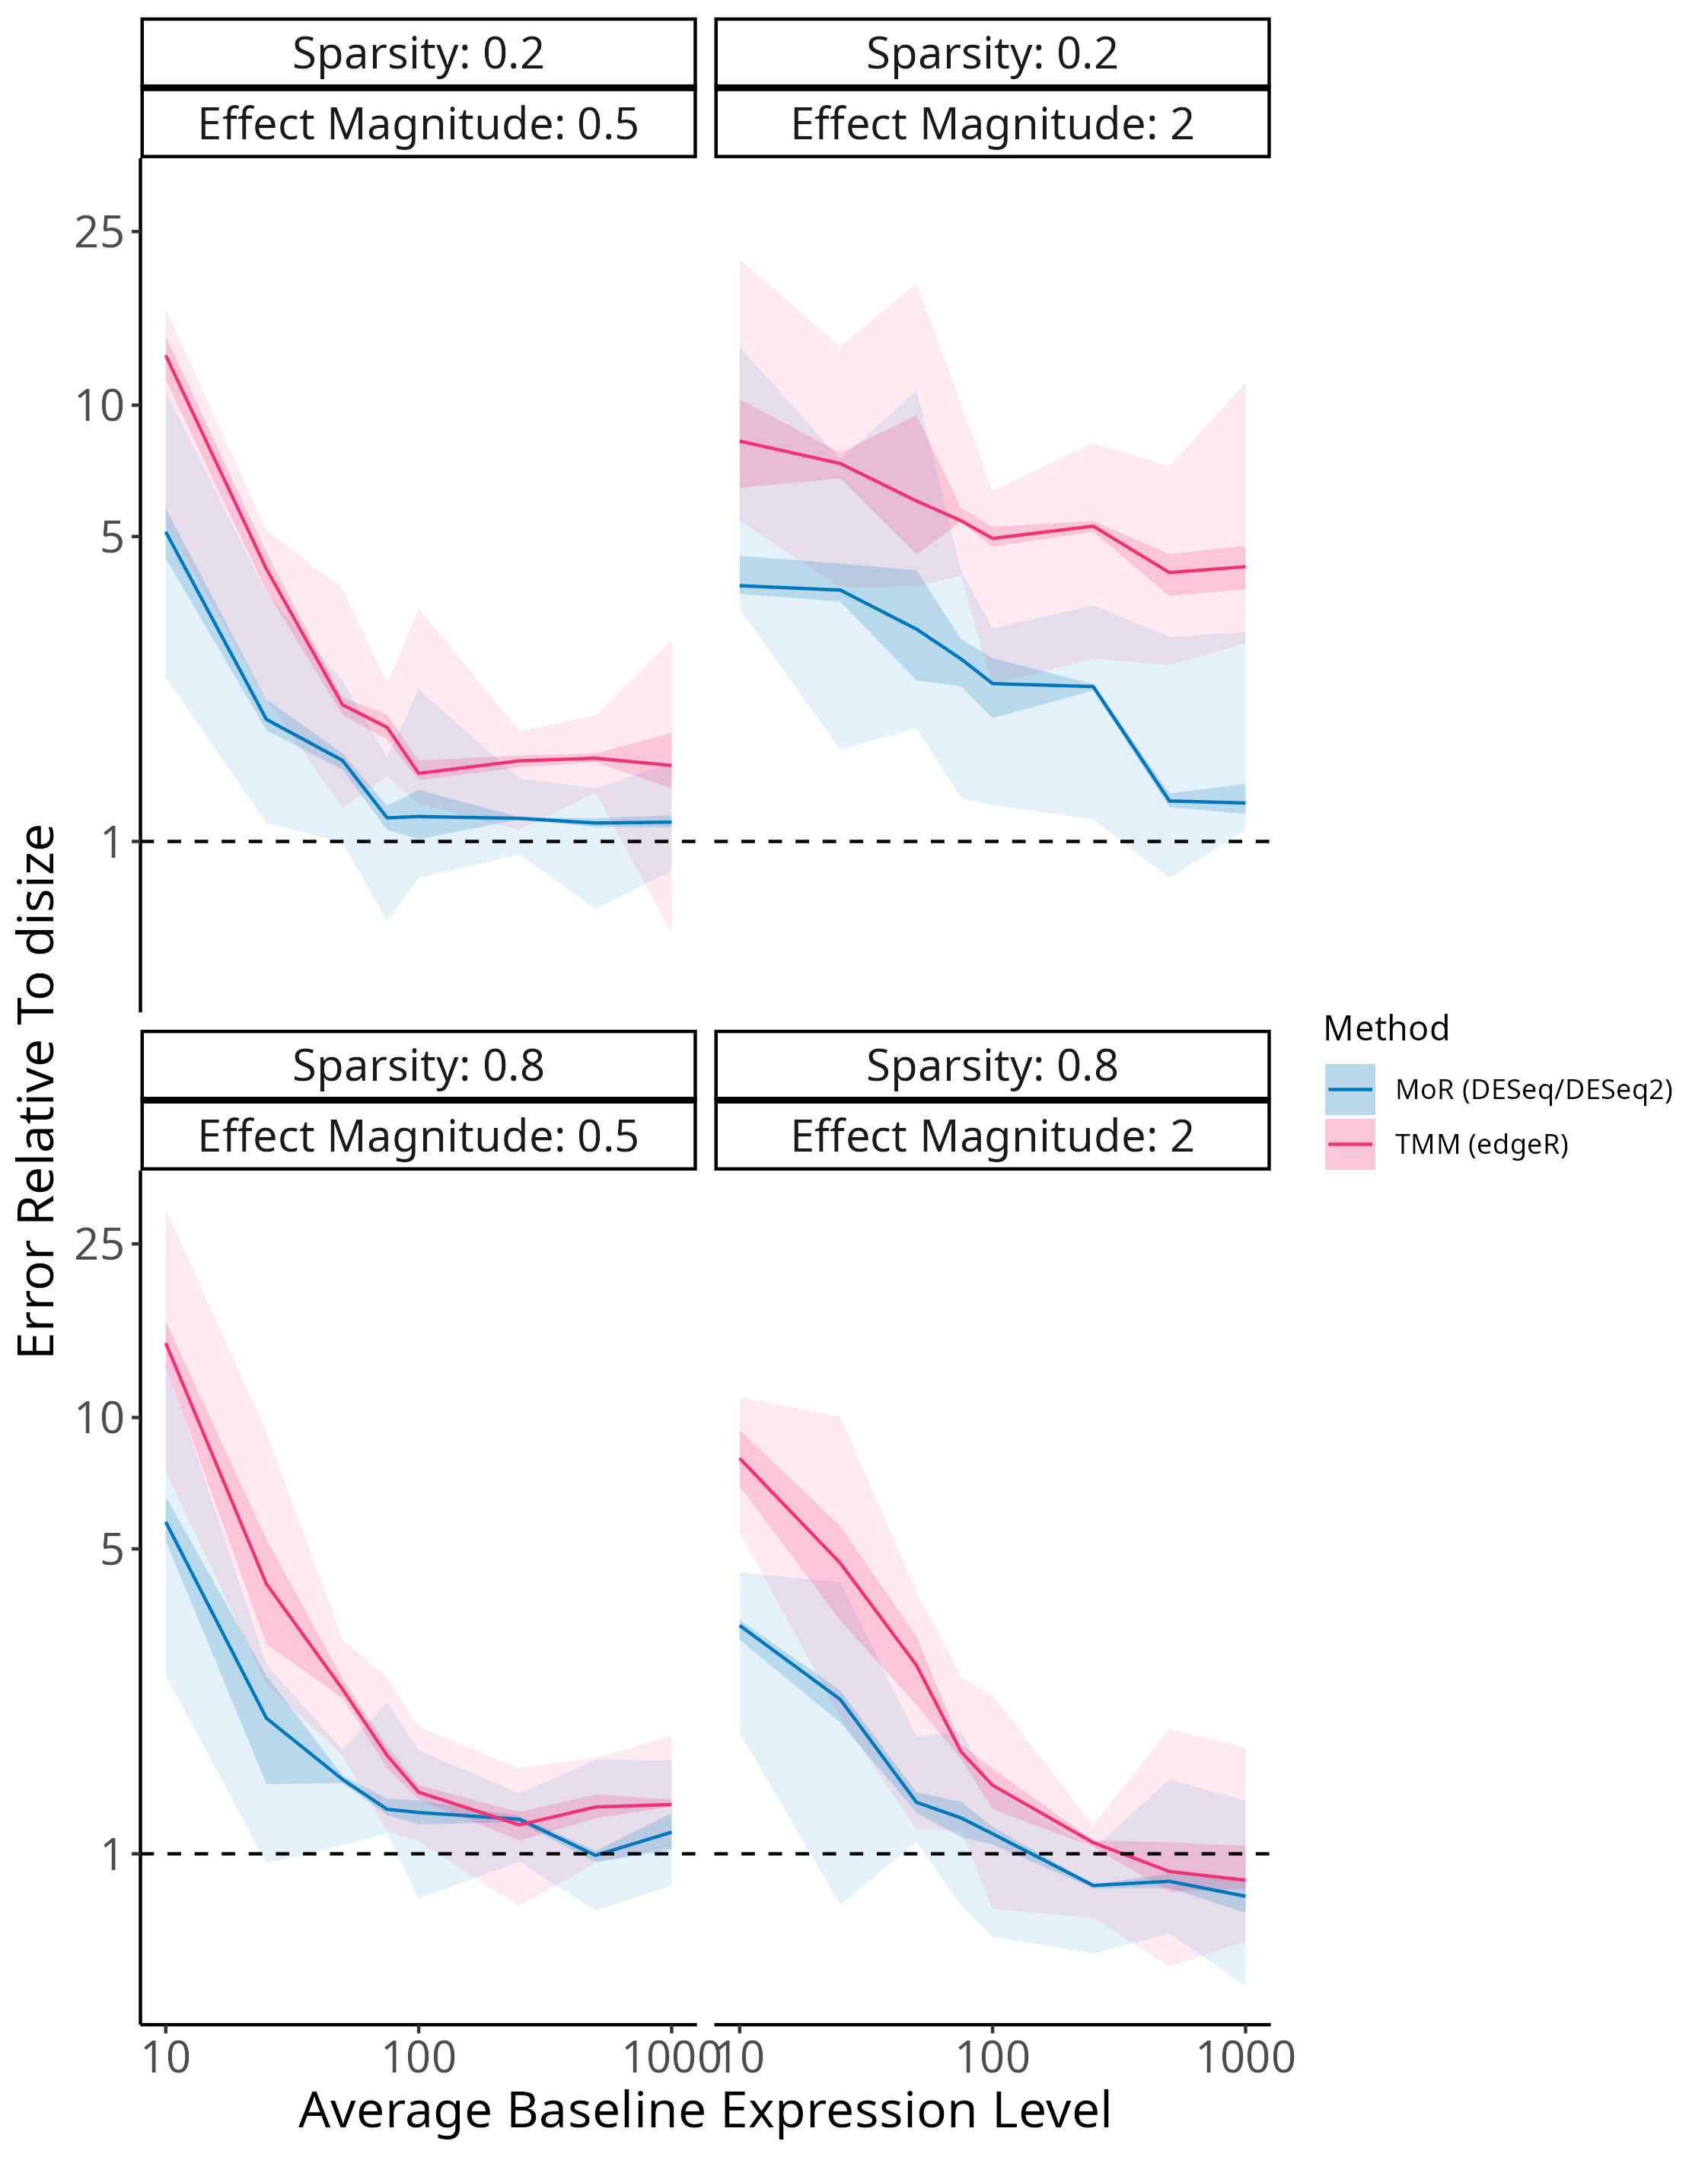
\includegraphics[width=\textwidth]{figures/suppfig-sfa-3.png}
\paragraph*{S3 Fig.}
\textbf{Comparing normalization methods for size factor accuracy in a multifactorial design.}
Fixing $n_g = 10000$ and varying $p$ and $\sigma$, relative size factor error of the other normalization methods (MoR and TMM) compared to \texttt{disize} versus the average baseline gene expression level. 
Each line represents the median relative error, while the shaded regions indicate the 5th-95th (lighter) and 40th-60th (darker) percentile ranges. 
A lower relative error indicates a more accurate size factor estimate.
\end{figure}

\begin{figure}[!ht]
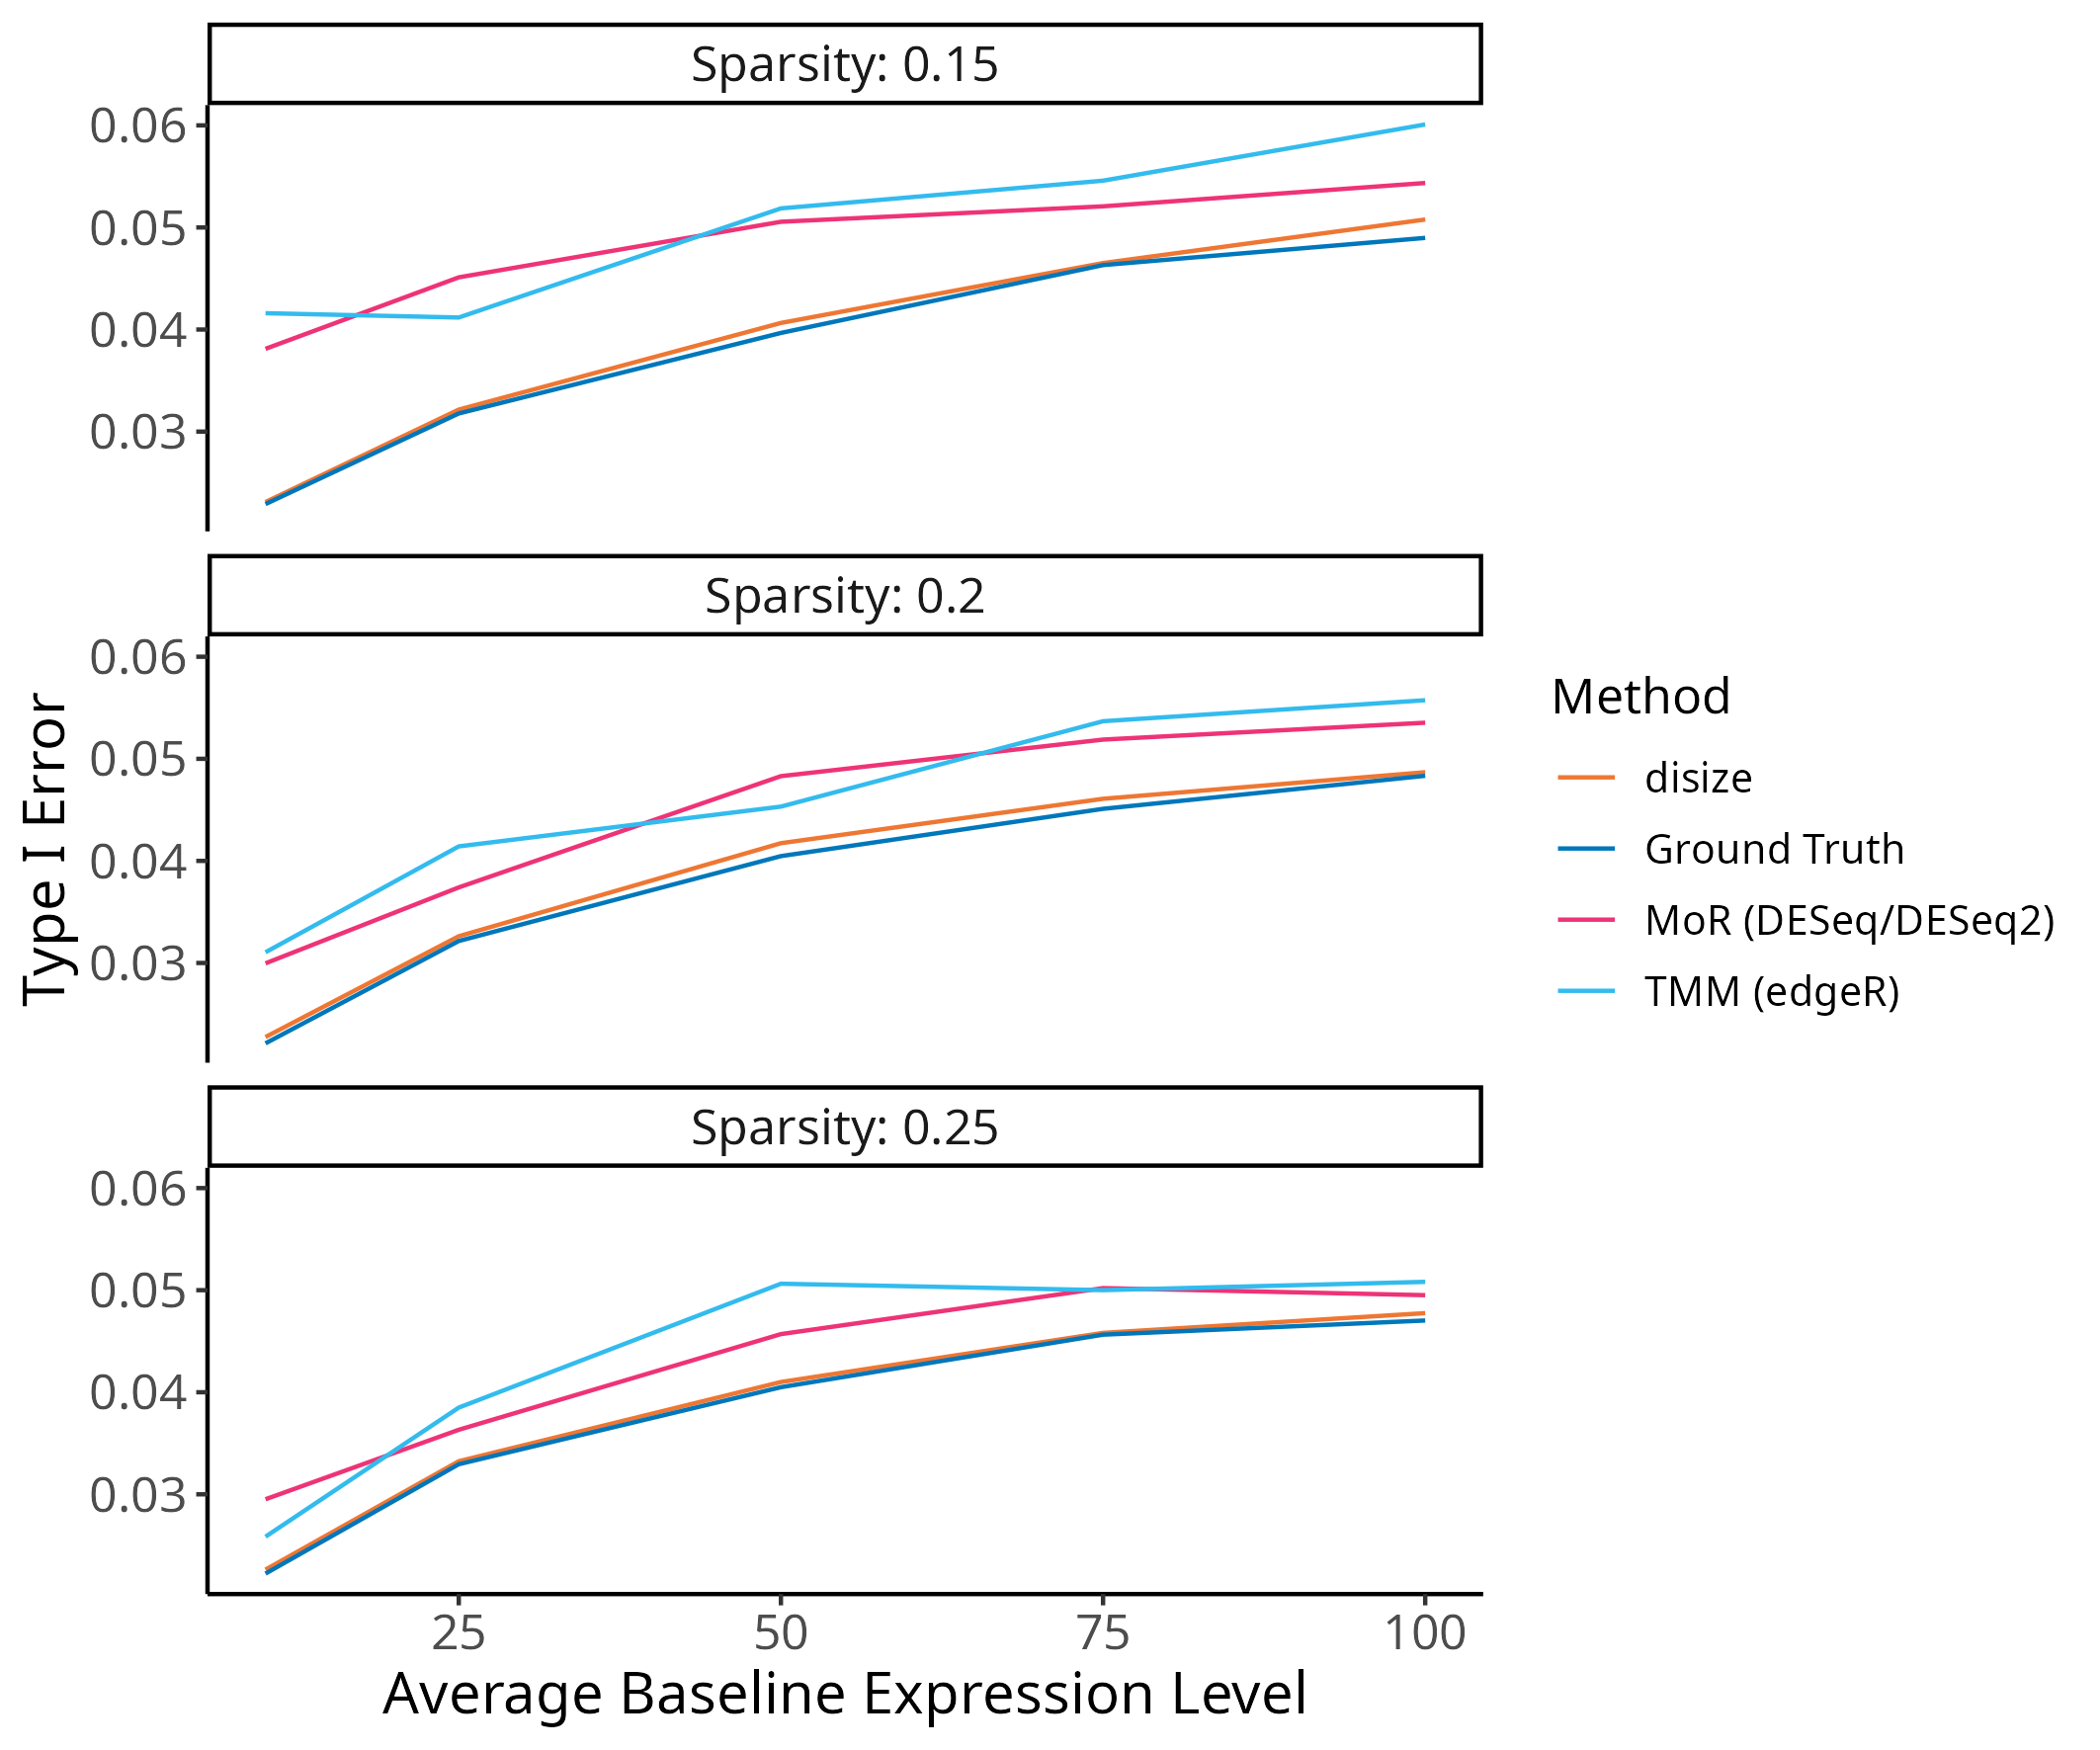
\includegraphics[width=\textwidth]{figures/suppfig-di-1.png}
\paragraph*{S4 Fig.}
\textbf{Comparing normalization methods for Type 1 error rates in a two-group design.}
Fixing $\alpha = 0.05$, $n_g = 10000$, $\sigma = 2$, and varying $p$, type 1 error rates of each normalization method (disize, MoR, and TMM) to the ground truth batch effect versus the average baseline gene expression level.
Values close to 1 are better.
\end{figure}

\begin{figure}[!ht]
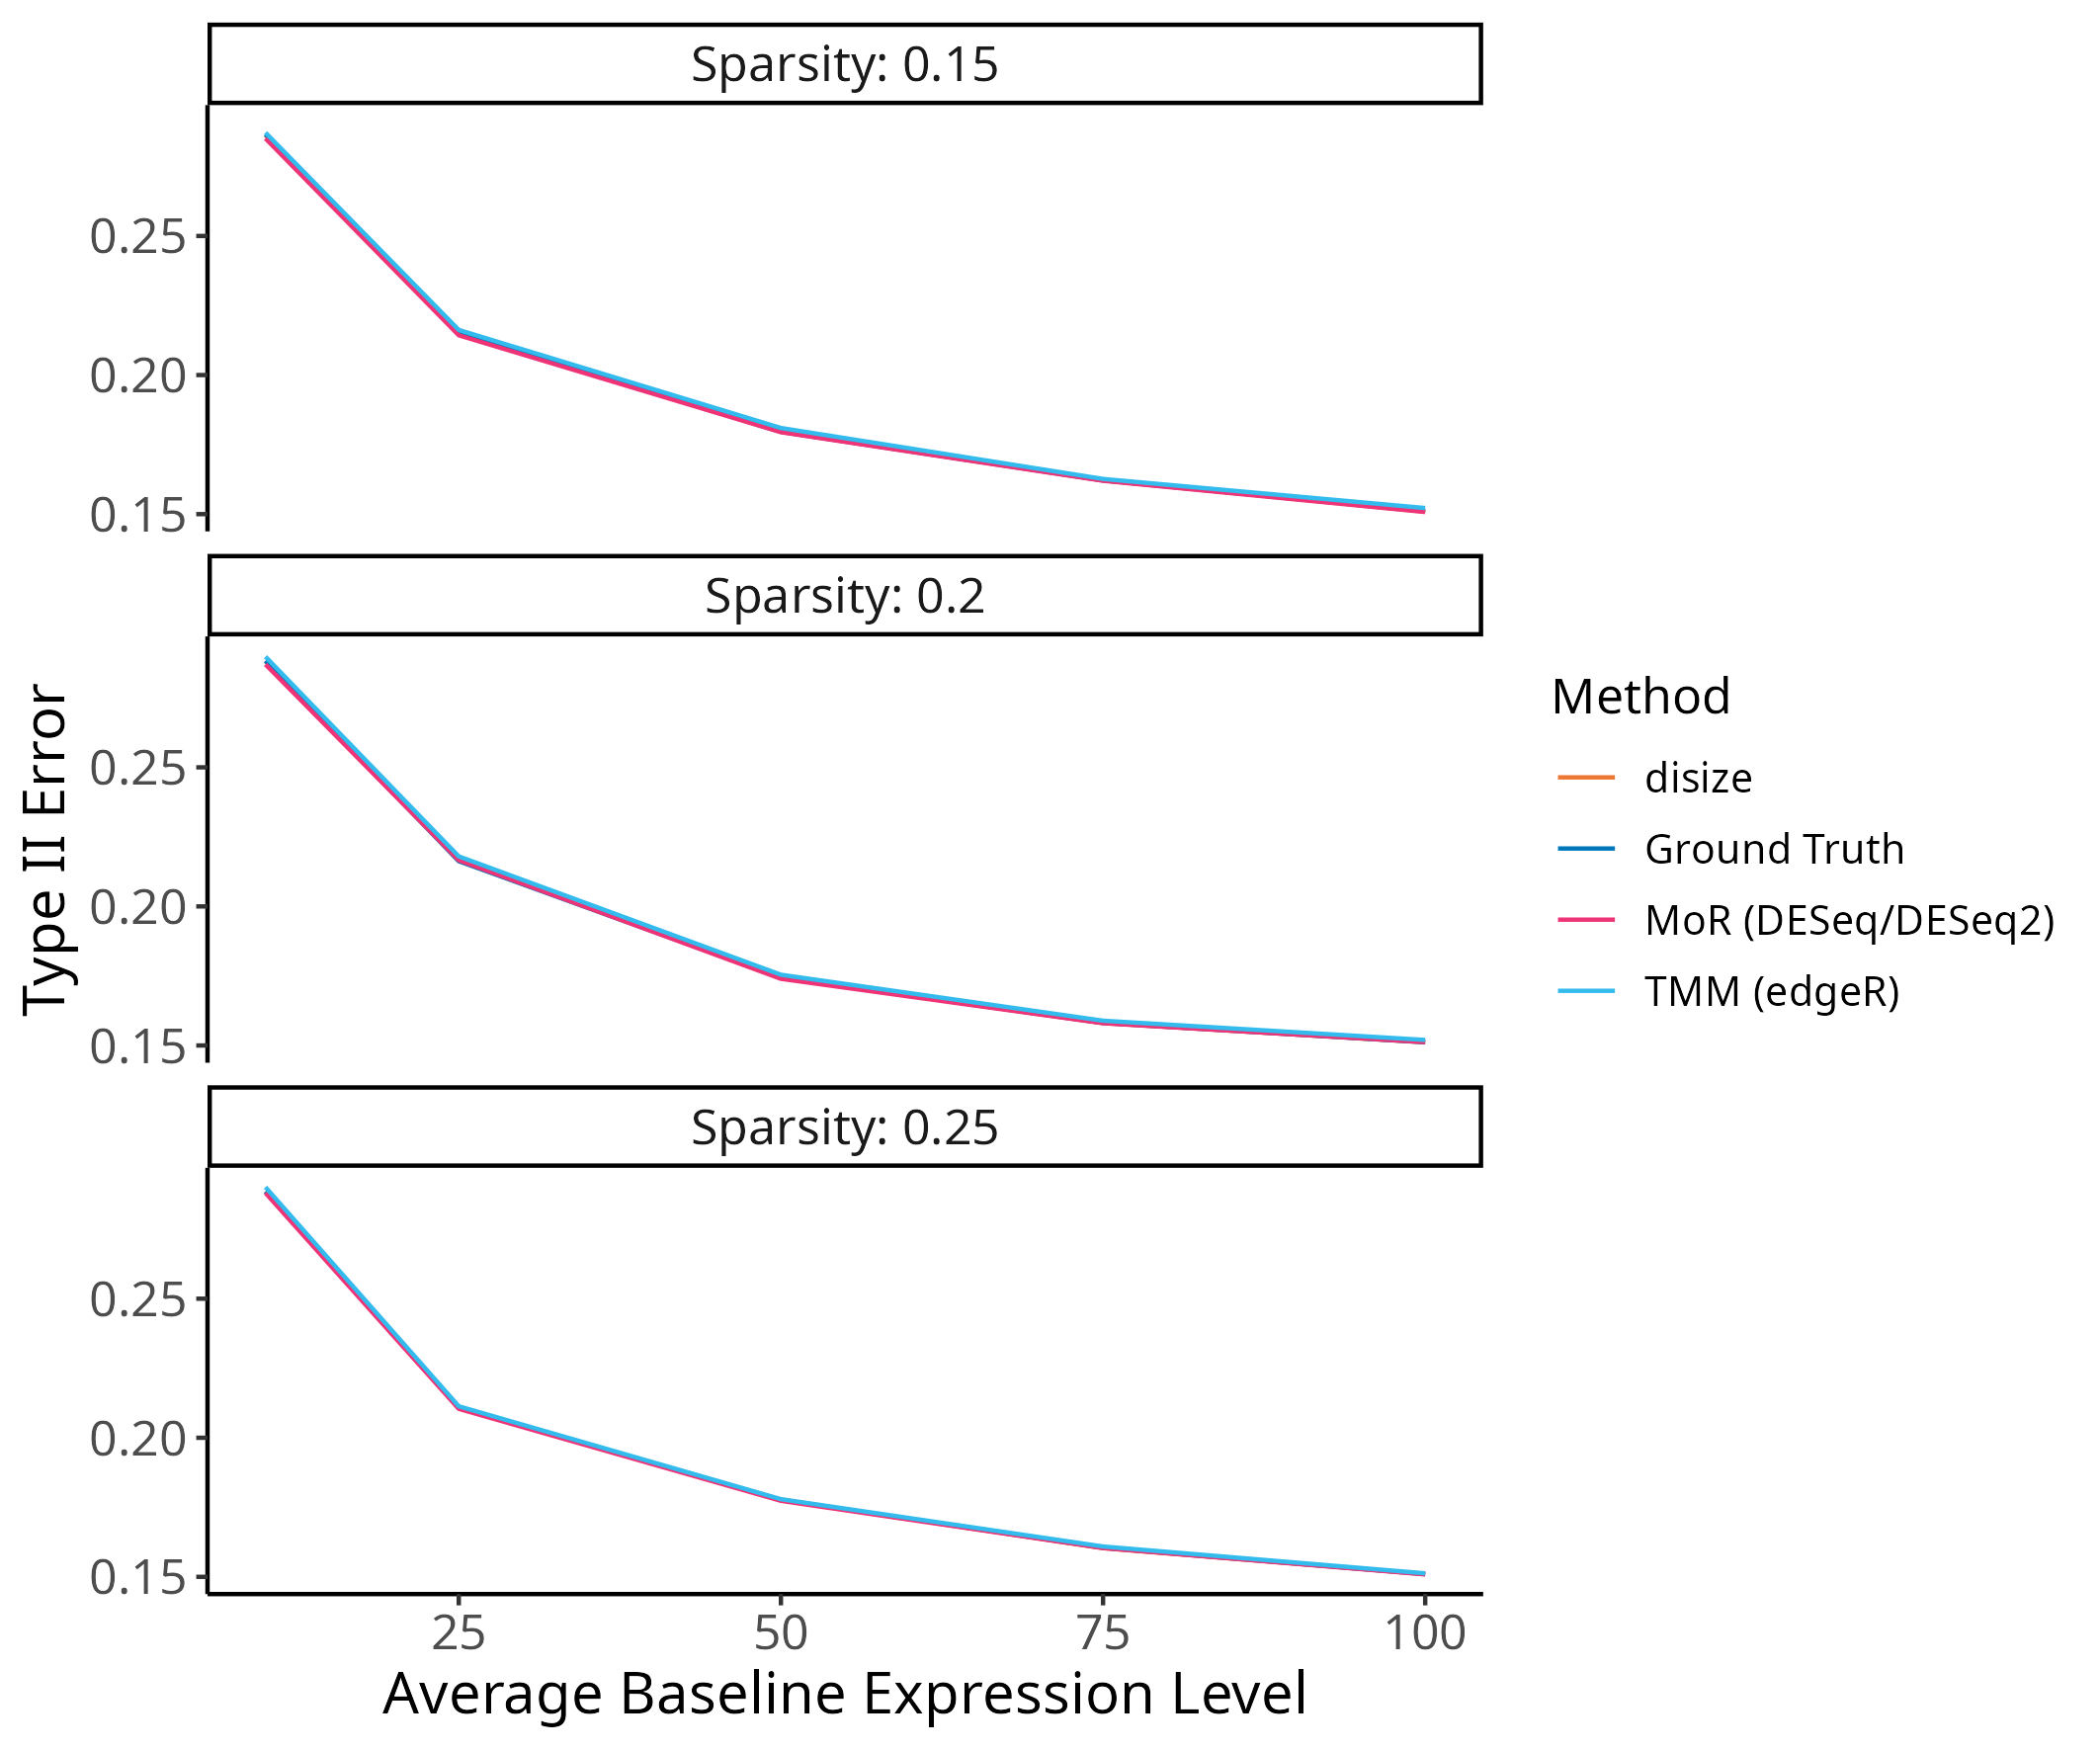
\includegraphics[width=\textwidth]{figures/suppfig-di-2.png}
\paragraph*{S5 Fig.}
\textbf{Comparing normalization methods for Type 2 error rates in a two-group design.}
Fixing $\alpha = 0.05$, $n_g = 10000$, $\sigma = 2$, and varying $p$, type 2 error rates of each normalization method (disize, MoR, and TMM) to the ground truth batch effect versus the average baseline gene expression level.
Values close to 1 are better.
\end{figure}

\section*{Acknowledgments}

\nolinenumbers

% Please compile your BiBTeX database using the "plos2025.bst" BibTeX style.
% This file is part of the current package.
% A sample BibTeX file is also included as "plos_bibtex_sample.bib".
%
% or
%
% Type in your references following Vancouver style and reference formatting instructions
% available at https://journals.plos.org/plosone/s/submission-guidelines#loc-references
% \begin{thebibliography}{}
% \bibitem{}
% Text
% \end{thebibliography}

\bibliography{disize}

\end{document}

